% CASCADED MAPS
Previously we discussed inferential transportation as firstly developed in \cite{Mapping:ElMoselhy2012,Mapping:Marzouk2016}.
Many more interesting ideas were proposed in the original literature, e.g.\ the composition of transport maps.
As a matter of fact, one does not need to transform the prior into the posterior in one step, which could possibly require a highly nonlinear map.
Instead, one might construct a sequence of maps that establish an appropriate coupling in a step-by-step manner,
i.e.\ one would only have to transport between similar interim distributions that progressively evolve into the target posterior.
This lowers the necessary degree of nonlinearity.
We do not investigate these ideas here, but focus on the one-step formulation.
\par % NUMERICAL EXPERIMENT
A numerical experiment is conducted in order to demonstrate and study the transformation method.
Its applicability for probabilistic parameter estimation is confirmed and its features and shortcomings are identified.
For these purposes, an inverse heat conduction problem (IHCP) \cite{Inversion:Wang2004,Inversion:Kaipio2011} is solved.
The setup is similar to the demonstration example used in the previous chapter.
After calling the problem to mind, a numerical demonstration of transformation-based Bayesian inference is given.
Markov chain Monte Carlo (MCMC) posterior sampling is employed as a reference and benchmarking solution.

\subsection{Problem setup}
% STEADY STATE HEAT CONDUCTION
We investigate a thermodynamic system with heat conduction in steady state, after a sufficiently long relaxation time has elapsed.
The stationary heat equation \(\nabla \cdot (\kappa \nabla \perfect{T}) = 0\) then governs the macroscopic diffusion of heat.
Let \(\tilde{T}(\bm{r})\) and \(\kappa(\bm{r})\) denote the fields of temperature and thermal conductivity, respectively.
They depend on the spatial coordinates \(\bm{r} = (r_1,r_2)^\top\).
Two space dimensions are considered.
\par % PROBLEM DOMAIN
A composite material with inclusions is the system under study.
An illustration of the system and its geometry is provided in \cref{fig:Transport:HeatConduction}.
% BOUNDARY CONDITIONS
The ``top'' of the domain is held at a fixed temperature \(\perfect{T}_1\), which establishes a first-type boundary condition.
At the ``bottom'' the heat flux \(q_2 = - \kappa_0 \, \partial \perfect{T} / \partial r_2\) through the boundary is prescribed, which imposes a second-type condition.
The ``left'' and ``right'' hand side are perfectly insulated such that there is no heat fluxing across the surfaces.
In \cref{tab:Transport:HeatConduction} the numeric values of the physical parameters including the boundary conditions are listed.
\par % FORWARD PROBLEM
While the thermal conductivity \(\kappa_0\) of the background matrix is considered well-known,
the \(\dimParam = 4\) conductivities \(\bm{\kappa} = (\kappa_1,\kappa_2,\kappa_3,\kappa_4)^\top\) of the material inclusions are the unknown parameters.
Their statistical inference is the goal of the Bayesian IHCP.
A number of \(\dimData = 16\) data points of the temperature \(\tilde{\bm{y}} = (\tilde{T}(\bm{r}_1),\ldots,\tilde{T}(\bm{r}_\dimData))^\top\)
at the sensor locations \((\bm{r}_1,\ldots,\bm{r}_\dimData)\) is measured and analyzed to that end.
The forward model \(\mathcal{M} \colon \bm{\kappa} \mapsto \tilde{\bm{y}}\) arises from solving the boundary value problem
corresponding to the partial differential equation for the measurable temperature as function of the unknowns.
Here, the finite element method is used together with an interpolation of the nodal values to the sensor locations.
A polynomial chaos expansion--based surrogate of the forward model is subsequently used in the Bayesian analysis.
% FIGURE & TABLE: PROBLEM SETUP
\begin{figure}[ht]
  \centering
  % FIGURE: HEAT CONDUCTION SETUP
  \begin{minipage}[c]{0.47\textwidth}
    \centering
    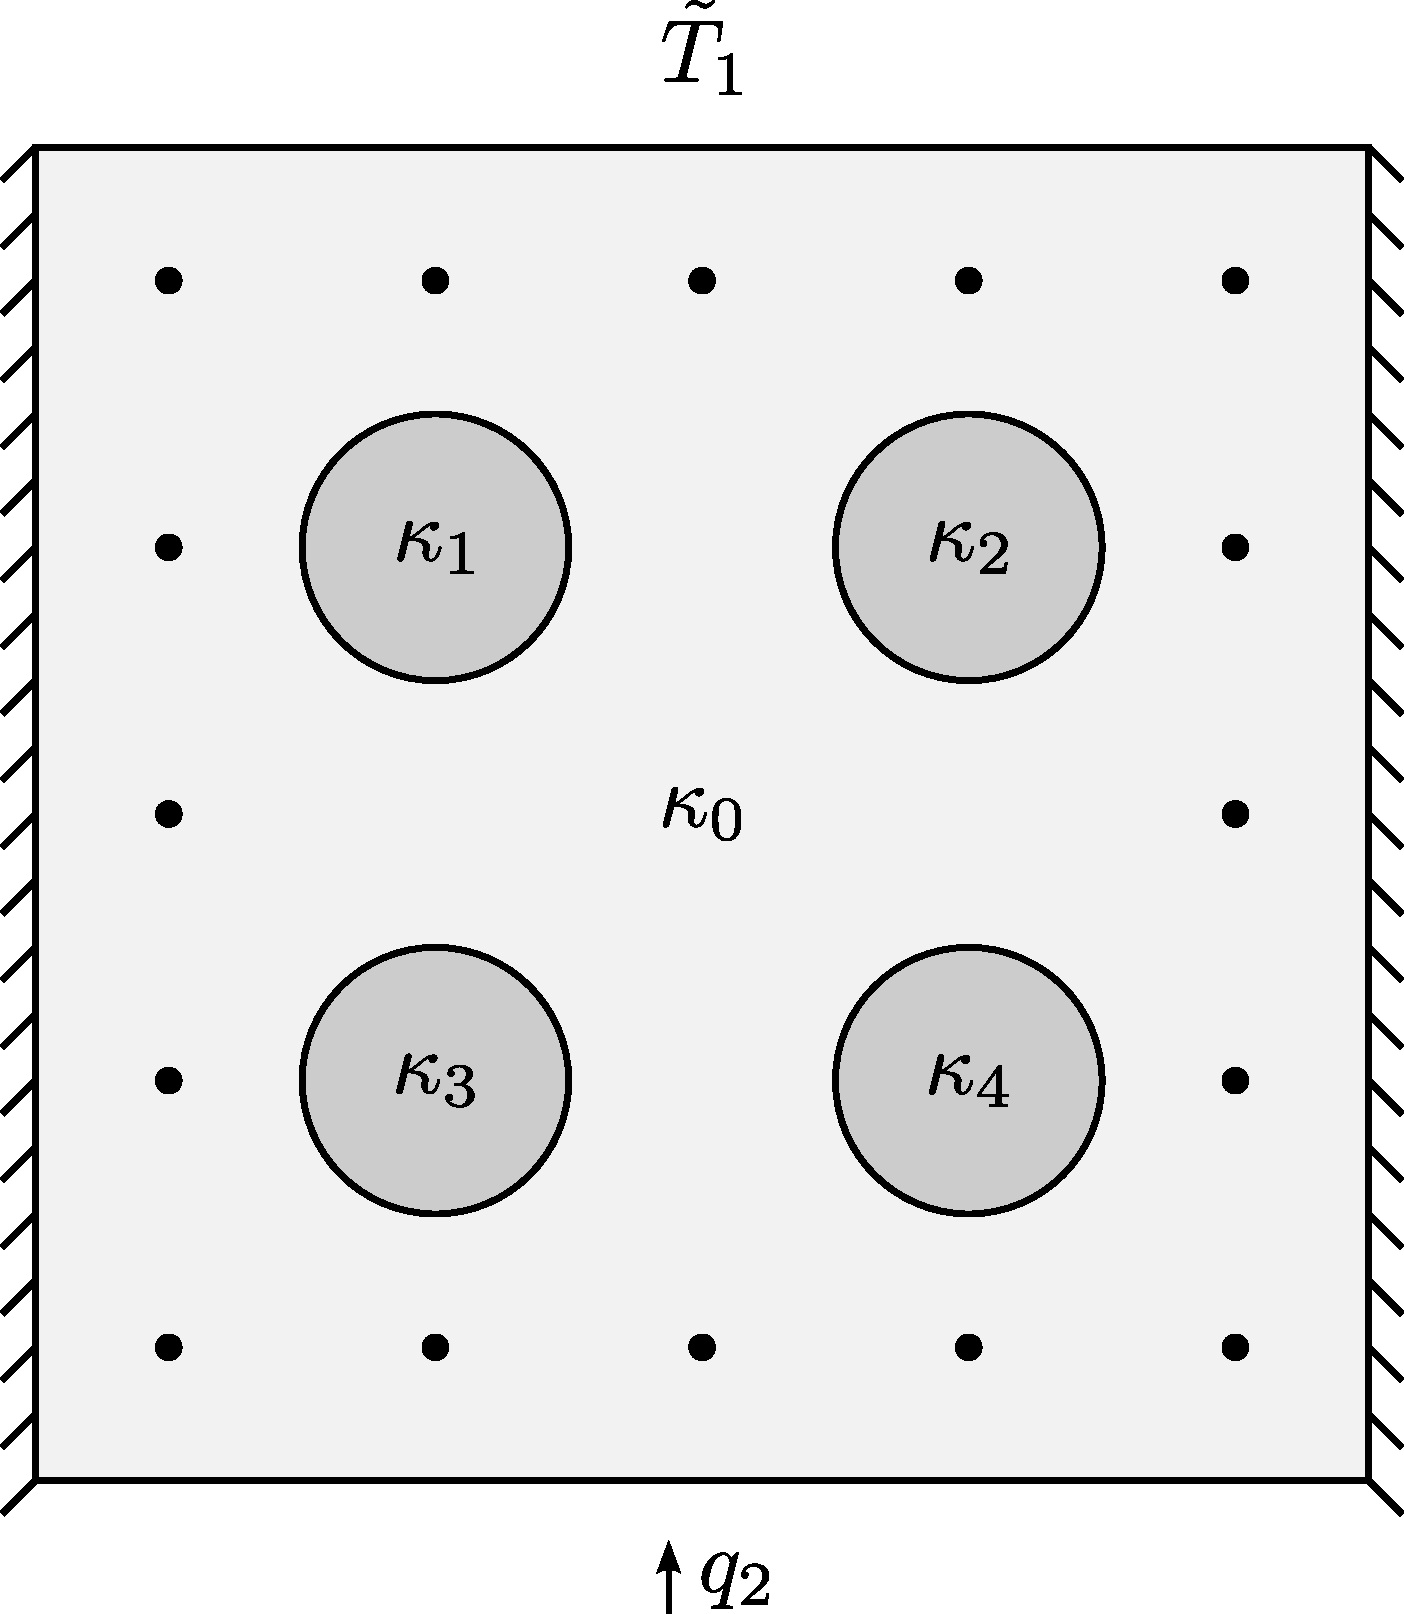
\includegraphics[height=\MAPfemHeight]{fig_Transport_HeatConduction}
    \captionof{figure}[Heat conduction setup]{Heat conduction setup.}
    \label{fig:Transport:HeatConduction}
  \end{minipage}%
  % TABLE: HEAT CONDUCTION SETUP
  \begin{minipage}[c]{0.53\textwidth}
    \captionof{table}[Numeric parameter values]{Numeric parameter values.}
    \label{tab:Transport:HeatConduction}
    \centering
    \begin{tabular}{ccccccc}
      \toprule
      \(\kappa_0\) & \(\kappa_1\) & \(\kappa_2\) & \(\kappa_3\) & \(\kappa_4\) & \(\tilde{T}_1\) & \(q_2\) \\
      \multicolumn{5}{c}{\([\unit[]{W/m/K}]\)} & \([\unit[]{K}]\) & \([\unit[]{W/m^2}]\) \\
      \midrule
      \(15\) & \(20\) & \(27\) & \(33\) & \(40\) & \(200\)& \(2000\) \\
      \bottomrule
    \end{tabular}
  \end{minipage}%
\end{figure}
\par % MEASUREMENT DATA (MODEL)
The data \(\bm{y} = (T(\bm{r}_1),\ldots,T(\bm{r}_\dimData))^\top\) comprise the observations of the temperature field at the measurement locations.
They are thought of as \(\bm{y} = \perfect{\bm{T}} + \bm{\varepsilon}\), i.e.\ as the model predictions \(\perfect{\bm{T}} = \mathcal{M}(\bm{\kappa})\) corrupted with noise \(\bm{\varepsilon}\).
A multivariate Gaussian distribution \(\pi(\bm{\varepsilon}) = \mathcal{N}(\bm{\varepsilon} \cond \bm{0},\bm{\Sigma})\) with mean \(\bm{0}\)
and covariance matrix \(\bm{\Sigma} = \sigma^2 \bm{I}\) represents the measurement noise.
The standard deviation \(\sigma\) quantifies the noise level.
It is specified as \(\sigma = \unit[0.25]{K}\) in the numerical experiment.
This establishes the data model \(\bm{Y} \cond \bm{\kappa} \sim \mathcal{N}(\bm{y} \cond \mathcal{M}(\bm{\kappa}),\sigma^2 \bm{I})\)
and the corresponding likelihood function \(\mathcal{L}(\bm{\kappa}) = \mathcal{N}(\bm{y} \cond \mathcal{M}(\bm{\kappa}),\sigma^2 \bm{I})\).
Herein we use pseudo-data that has been simulated according to the probability model just described.
\par % PRIOR DENSITY
We select a multivariate Gaussian prior distribution \(\pi(\bm{\kappa}) = \prod_{i=1}^4 \pi(\kappa_i)\) with independent marginals \(\pi(\kappa_i) = \mathcal{N}(\kappa_i \cond \mu_0,\sigma_0^2)\).
The mean and standard deviations are respectively specified as \(\mu_0 = \unit[30]{W/m/K}\) and \(\sigma_0 = \unit[5]{W/m/K}\).
% NEGATIVE CONDUCTIVITIES
Even though this prior setup allows for negative thermal conductivities in principle, they are six standard deviations far away from the mean.
The prior probability mass assigned to those unphysical values is thus negligibly small.
% POSTERIOR DENSITY
After the IHCP setup has been finally completed,
for the density of the posterior distribution one has \(\pi(\bm{\kappa} \cond \bm{y}) = \scale^{-1} \mathcal{L}(\bm{\kappa}) \pi(\bm{\kappa})\).

\subsection{Algorithmic implementation}
% BFGS ALGORITHM
As already mentioned, many techniques from nonlinear programming \cite{Optim:Bazaraa2006,Optim:Sun2006,Optim:Zornig2014} are now readily available
for computing the posterior distribution by transforming the prior appropriately.
We employ a quasi-Newton method where, in general black-box fashion, the necessary derivatives are smartly calculated by finite-differencing.
In particular, we use the \emph{Broyden--Fletcher--Goldfarb--Shanno} (BFGS) \emph{algorithm} \cite{Optim:Broyden1970:a,Optim:Broyden1970:b,Optim:Fletcher1970,Optim:Goldfarb1970,Optim:Shanno1970},
an iterative quasi-Newton method for unconstrained nonlinear optimization.
It is arguably one of the most widespread algorithms for this type of programming problems.
\par % OTHER OPTIMIZERS
Several other local and global optimizers were tried out.
This involves derivative-free optimization algorithms such as the Nelder--Mead method and pattern search.
Moreover, this includes techniques from evolutionary computing such as a genetic algorithm, particle swarm optimization and the covariance matrix adaption evolution strategy.
A typology of these diverse approaches eludes the scope of this chapter.
The interested reader is redirected to \cite{Optim:Nocedal2006,Optim:Eiben2015} for comprehensive overviews.
As compared to BFGS, the performance of these techniques turns out to be rather mediocre.
Hence, the BFGS algorithm is selected.
\par % ALGORITHMIC PARAMETERS
Multivariate normalized Hermite polynomials in conjunction with a standardizing parameter transform are used to build the triangular map.
In order to avoid a too complex notation, the linear reparametrization remains implicit in the discussion of the inferential coupling.
The sample average utility function is maximized as in \cref{eq:Transport:OptimizationSAA} in a series of preliminary runs,
where different values of \(K\) in \cref{eq:Transport:SampleAverageFunction} and \(p\) in \cref{eq:Transport:PolynomialMap} are tested.
Apart from the comparison with the results from MCMC simulation, which hardly establishes a stand-alone solution,
the only criterion at hand for deciding on those parameters is that the variance of \cref{eq:Transport:Lambda} should be minimal as in \cref{eq:Transport:OptimizationLambda}.
On this basis, we eventually choose a rather high sample size \(K = 10^5\) for the SAA and a very low maximal polynomial degree \(p = 2\).
According to \cref{eq:Transport:Cardinality} we then have to find \(P = 34\) unknown coefficients \(\bm{\coeffM}\) of the transport map \(\map_{\bm{\coeffM}}^\vartriangle(\bm{x})\).
\par % ALGORITHM START/STOP
The BFGS algorithm is initialized at the identity map.
It starts from the values \(\bm{\coeffM}_0\) for which \(\map_{\bm{\coeffM}_0}^\vartriangle(\bm{x}) = \bm{x}\) is the identity map and then,
over the course of the optimization, gradually transforms the prior into the posterior.
It is stopped after \(I = 51\) iterations and roughly three hours of program runtime,
when the first-order optimality criterion \(\lVert \nabla \hat{\mathcal{G}}(\bm{\coeffM}_I) \rVert_\infty \leq 10^{-6}\) is fulfilled.
The final estimates of the coefficients that determine the inferential map \(\map_{\hat{\bm{\coeffM}}}^\vartriangle(\bm{x})\) are given as \(\hat{\bm{\coeffM}} = \bm{\coeffM}_I\).
We obtain \(\hat{\mathcal{G}}(\hat{\bm{\coeffM}}) = -9.22\) and \(\exp(\hat{\mathcal{G}}(\hat{\bm{\coeffM}})) = 9.86 \times 10^{-5}\) for the maximal value of the utility and its exponential.
% CONVERGENCE CHECKS
In \cref{tab:Transport:BFGS:Convergence} the quantities \(\exp(\hat{\mathcal{G}}(\bm{\coeffM}_\iota))\) and \(\mathrm{Var}[\Lambda_{\bm{\coeffM}_\iota}(\bm{X})]\)
are listed for the intermediate values of the coefficients \(\bm{\coeffM}_\iota\) that are obtained after every tenth iteration \(\iota \in \{0,1,10,20,30,40,50\}\).
While the evidence-related quantity \(\exp(\hat{\mathcal{G}}(\bm{\coeffM}_\iota))\) is maximized, \(\mathrm{Var}[\Lambda_{\bm{\coeffM}_\iota}(\bm{X})]\) is a separate convergence indicator.
It attains \(\mathrm{Var}[\Lambda_{\hat{\bm{\coeffM}}}(\bm{X})] = 0.73\) in the last iteration.
% TABLE: ASSESSING CONVERGENCE
\begin{table}[htbp]
  \caption[BFGS optimization]{BFGS optimization.}
  \label{tab:Transport:BFGS:Convergence}
  \centering
  \resizebox{\linewidth}{!}{
  \begin{tabular}{llllllll}
    \toprule
    Iteration no.\ \(\iota\) & \multicolumn{1}{c}{\(0\)} & \multicolumn{1}{c}{\(1\)} & \multicolumn{1}{c}{\(10\)}
    & \multicolumn{1}{c}{\(20\)} & \multicolumn{1}{c}{\(30\)} & \multicolumn{1}{c}{\(40\)} & \multicolumn{1}{c}{\(50\)} \\
    \midrule
    \(\exp(\hat{\mathcal{G}}(\bm{\coeffM}_\iota))\)
    & \(4.23 \times 10^{-86}\) & \(1.48 \times 10^{-58}\) & \(3.25 \times 10^{-5}\) & \(9.63 \times 10^{-5}\) & \(9.86 \times 10^{-5}\) & \(9.86 \times 10^{-5}\) & \(9.86 \times 10^{-5}\) \\
    \(\mathrm{Var}[\Lambda_{\bm{\coeffM}_\iota}(\bm{X})]\)
    & \(2.44 \times 10^{4}\) & \(1.08 \times 10^{4}\) & \(6.71 \times 10^{0}\) & \(8.52 \times 10^{-1}\) & \(7.29 \times 10^{-1}\) & \(7.31 \times 10^{-1}\) & \(7.31 \times 10^{-1}\) \\
    \bottomrule
  \end{tabular}
  }
\end{table}
\par % CONVERGENCE OF THE COEFFICIENTS
It is interesting to monitor the convergence of the coefficients over the BFGS iterations.
In \cref{fig:Transport:BFGS:Coefficients} the components of the coefficient vector \(\bm{\coeffM}_\iota\) are shown for \(\iota = 0,\ldots,50\).
The constant, linear and quadratic terms can be distinguished by their color.
As it can be seen, the coefficients have almost reached their final values after about ten to twenty iterations and hardly change thereafter.
Accordingly, we could have stopped the algorithm at this point already.
Notice that the constant terms, which establish the posterior mean vector, start from the prior means and then approach the true values of the unknown thermal conductivities.
The remaining coefficients of the linear and quadratic terms concentrate around lower values.
They determine further characteristics of the posterior distribution such as the variances and correlations.
% FIGURE: BFGS COEFFICIENTS
\begin{figure}[htbp]
  \centering
  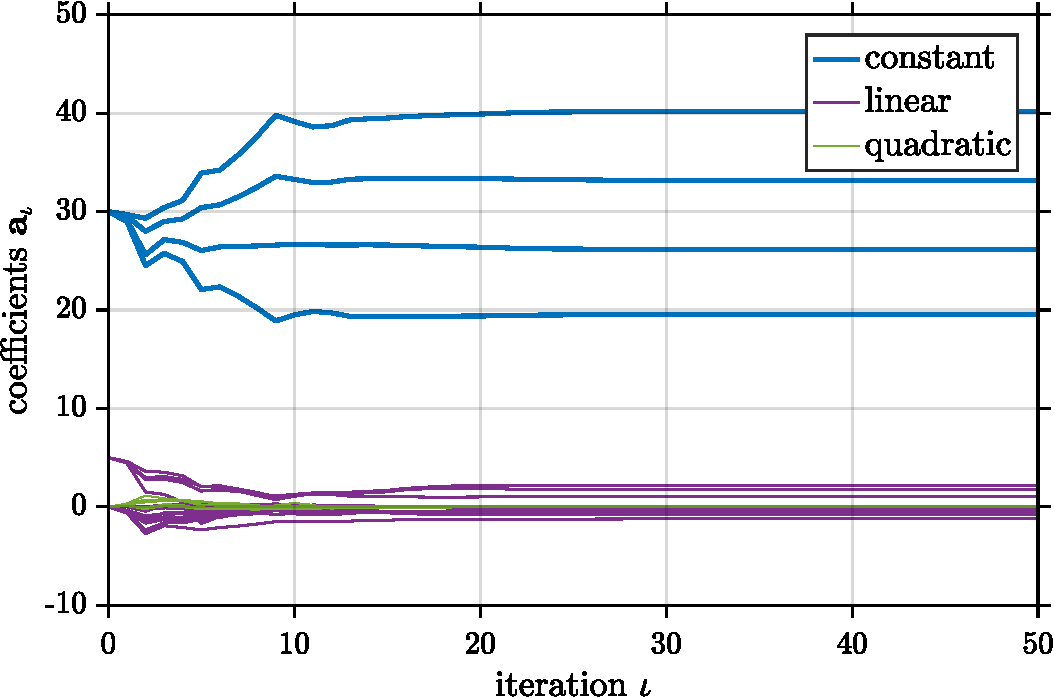
\includegraphics[height=\MAPfigHeight]{fig_Transport_BFGS_Coefficients}
  \caption[Converging coefficients]{Converging coefficients.}
  \label{fig:Transport:BFGS:Coefficients}
\end{figure}
\par % CONVERGENCE OF THE MOMENTS
The means and \(\mathds{E}[\kappa_i \cond \bm{y}]\) standard deviations \(\mathrm{Std}[\kappa_i \cond \bm{y}] = \mathrm{Var}[\kappa_i \cond \bm{y}]^{1/2}\)
of the posterior distribution for \(i = 1,2,3,4\) over the first twenty BFGS iterations are listed in \cref{tab:Transport:BFGS:Moments}.
After every second algorithm iteration, the current values of the optimization parameters are used in the calculation
of the two first posterior moments according to \cref{eq:Transport:OutputMeanVariance,eq:Transport:OutputCovariance}.
As it is observed, the expected values of the transformed random variables evolve from the prior into the posterior means.
At the same time, the standard deviations expectedly decrease from the prior to the posterior level.
The final estimates of the discussed posterior characteristics are further analyzed below.
% TABLE: BFGS MOMENTS
\begin{table}[htbp]
  \caption[Converging moments]{Converging moments.}
  \label{tab:Transport:BFGS:Moments}
  \centering
  \begin{tabular}{rcrrrrrrrrrrr}
    \toprule
    \multicolumn{2}{l}{Iteration no.\ \(\iota\)} & \multicolumn{1}{c}{\(0\)} & \multicolumn{1}{c}{\(2\)} & \multicolumn{1}{c}{\(4\)}
    & \multicolumn{1}{c}{\(6\)} & \multicolumn{1}{c}{\(8\)} & \multicolumn{1}{c}{\(10\)} & \multicolumn{1}{c}{\(12\)}
    & \multicolumn{1}{c}{\(14\)} & \multicolumn{1}{c}{\(16\)} & \multicolumn{1}{c}{\(18\)} & \multicolumn{1}{c}{\(20\)} \\
    \midrule
    \(\mathds{E}[\kappa_1 \cond \bm{y}]\) & \multirow{4}{*}{\rotatebox[origin=c]{270}{\([\unit[]{W/m/K}]\)}}
    & \(30\) & \(24.52\) & \(24.93\) & \(22.35\) & \(20.19\) & \(19.49\) & \(19.71\) & \(19.34\) & \(19.35\) & \(19.36\) & \(19.39\) \\
    \(\mathds{E}[\kappa_2 \cond \bm{y}]\) &
    & \(30\) & \(25.61\) & \(26.87\) & \(26.41\) & \(26.51\) & \(26.67\) & \(26.59\) & \(26.61\) & \(26.55\) & \(26.46\) & \(26.38\) \\
    \(\mathds{E}[\kappa_3 \cond \bm{y}]\) &
    & \(30\) & \(28.00\) & \(29.25\) & \(30.68\) & \(32.48\) & \(33.27\) & \(32.99\) & \(33.33\) & \(33.35\) & \(33.35\) & \(33.34\) \\
    \(\mathds{E}[\kappa_4 \cond \bm{y}]\) &
    & \(30\) & \(29.32\) & \(31.13\) & \(34.22\) & \(37.64\) & \(39.15\) & \(38.72\) & \(39.42\) & \(39.64\) & \(39.79\) & \(39.90\) \\
    \midrule
    \(\mathrm{Std}[\kappa_1 \cond \bm{y}]\) & \multirow{4}{*}{\rotatebox[origin=c]{270}{\([\unit[]{W/m/K}]\)}}
    & \(5\) & \(3.38\) & \(3.05\) & \(2.33\) & \(1.53\) & \(1.23\) & \(1.33\) & \(1.16\) & \(1.11\) & \(1.10\) & \(1.10\) \\
    \(\mathrm{Std}[\kappa_2 \cond \bm{y}]\) &
    & \(5\) & \(4.31\) & \(2.88\) & \(2.60\) & \(1.97\) & \(1.80\) & \(1.82\) & \(1.59\) & \(1.58\) & \(1.57\) & \(1.57\) \\
    \(\mathrm{Std}[\kappa_3 \cond \bm{y}]\) &
    & \(5\) & \(3.65\) & \(3.21\) & \(2.05\) & \(1.17\) & \(1.08\) & \(1.41\) & \(1.44\) & \(1.74\) & \(1.90\) & \(1.89\) \\
    \(\mathrm{Std}[\kappa_4 \cond \bm{y}]\) &
    & \(5\) & \(3.43\) & \(2.93\) & \(2.04\) & \(1.50\) & \(1.38\) & \(1.59\) & \(1.66\) & \(1.94\) & \(2.15\) & \(2.22\) \\
    \bottomrule
  \end{tabular}
\end{table}

\subsection{Posterior distribution}
% INDEPENDENT POSTERIOR SAMPLING
After an appropriate random variable transformation has been found, the posterior distribution can be analyzed in view of its marginals, statistical moments and the like.
The most general way of doing so is to sample the posterior.
To that end one draws independent samples from the prior and applies the computed transformation to each of them individually.
Independent samples from the posterior result from this procedure.
They can be subsequently analyzed in order to visualize the posterior marginals or to compute conditional expectation values.
\par % ONE-DIMENSIONAL POSTERIOR MARGINALS
For the analysis of the marginal distributions, a prior sample of the size \(L = 10^7\) is used.
The same total number of samples is also computed by means of MCMC with thirty parallel chains.
A comparison of the four posterior marginals is found in \cref{fig:Transport:Post:Marginals1D}.
In \cref{fig:Transport:Post:Marginals1D:MCMC} histograms of the obtained MCMC sample are depicted.
Directly besides in \cref{fig:Transport:Post:Marginals1D:Map} histograms of the map-based posterior marginals are plotted.
As far as one can tell by visual inspection, the marginals obtained from both methods are nearly identical.
Only a minor deviation shows up in the fourth marginal.
This means that the posterior marginals are captured very well with a low-degree triangular transformation.
% FIGURES: ONE-DIMENSIONAL POSTERIOR MARGINALS
\begin{figure}[htbp]
  \centering
  \begin{subfigure}[b]{\MAPsubWidth}
    \centering
    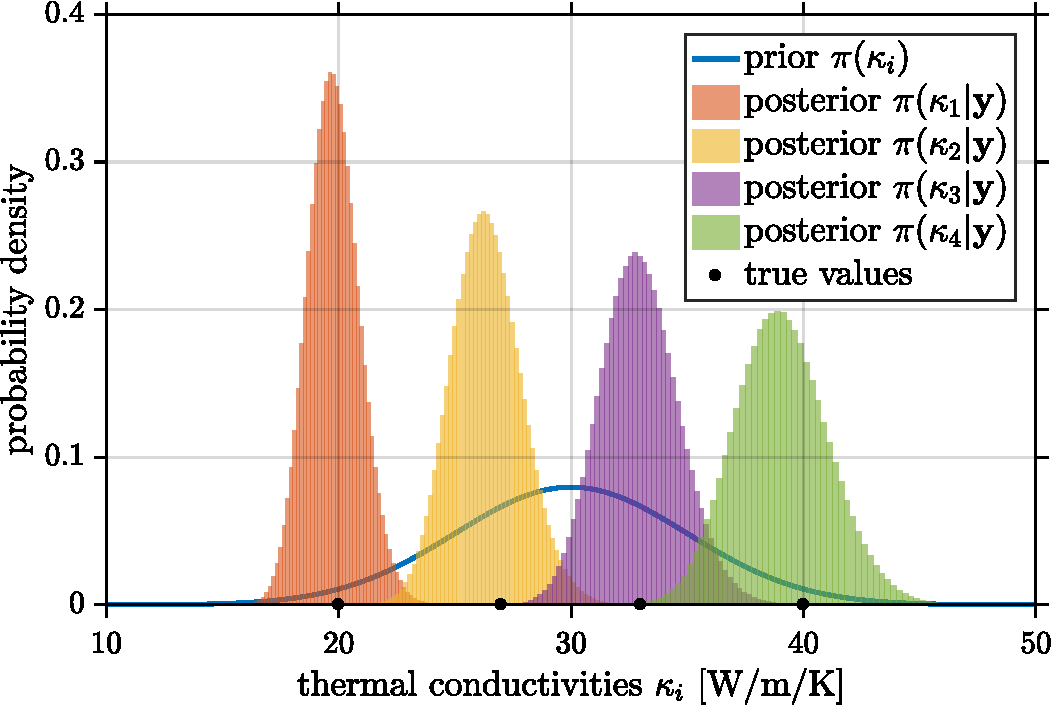
\includegraphics[height=\MAPfigHeight]{fig_Transport_Post1D_MCMC}
    \caption{MCMC.}
    \label{fig:Transport:Post:Marginals1D:MCMC}
  \end{subfigure}\hfill%
  \begin{subfigure}[b]{\MAPsubWidth}
    \centering
    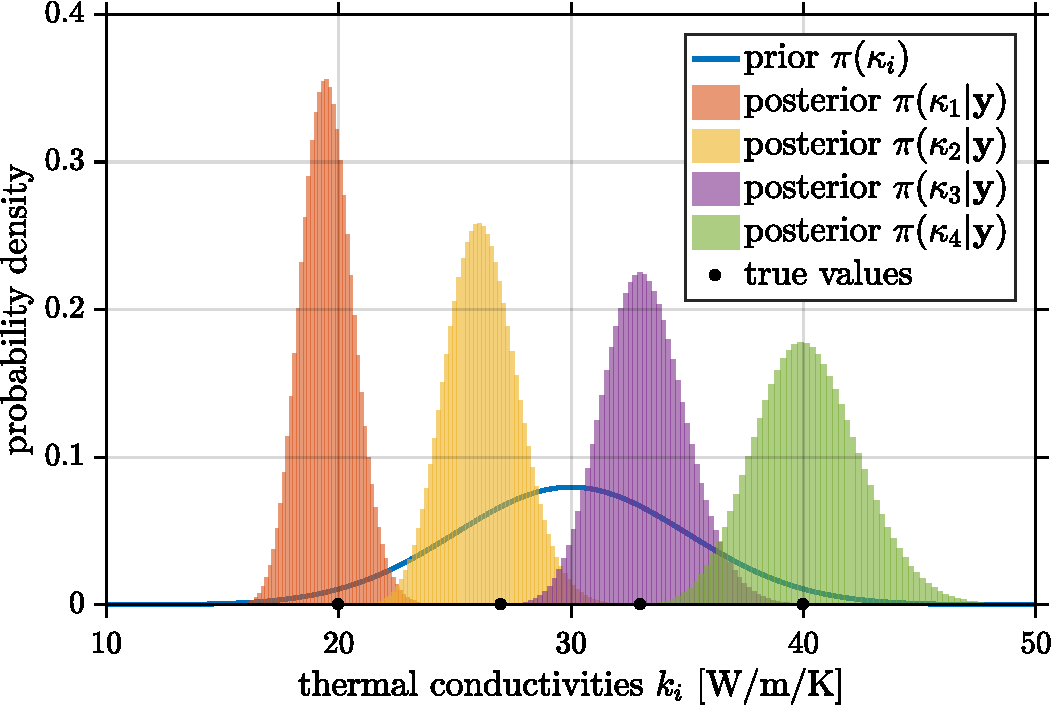
\includegraphics[height=\MAPfigHeight]{fig_Transport_Post1D_Map}
    \caption{Mapping.}
    \label{fig:Transport:Post:Marginals1D:Map}
  \end{subfigure}%
  \caption[One-dimensional posterior marginals]{One-dimensional posterior marginals.}
  \label{fig:Transport:Post:Marginals1D}
\end{figure}
\par % TWO-DIMENSIONAL MARGINALS
We also investigate some of the two-dimensional posterior marginals.
A collection of bivariate histograms of those marginals can be found in \cref{fig:Transport:Post:Marginals2D}.
The results obtained from MCMC sampling are located on the left side, the ones from the prior transformation are shown on the right.
In \cref{fig:Transport:Post:Marginals2D:12:MCMC,fig:Transport:Post:Marginals2D:12:Map} the marginal \(\pi(\kappa_1,\kappa_2 \cond \bm{y})\) is visualized.
Similarly, \cref{fig:Transport:Post:Marginals2D:23:MCMC,fig:Transport:Post:Marginals2D:23:Map} contain \(\pi(\kappa_2,\kappa_3 \cond \bm{y})\)
while \cref{fig:Transport:Post:Marginals2D:34:MCMC,fig:Transport:Post:Marginals2D:34:Map} show \(\pi(\kappa_3,\kappa_4 \cond \bm{y})\).
Transformation-based inference leads to two-dimensional posterior marginals that seem to be slightly flattened out as compared to their MCMC solutions.
% FIGURES: TWO-DIMENSIONAL POSTERIOR MARGINALS
\begin{figure}[htbp]
  \centering
  \begin{subfigure}[b]{\MAPsubWidth}
    \centering
    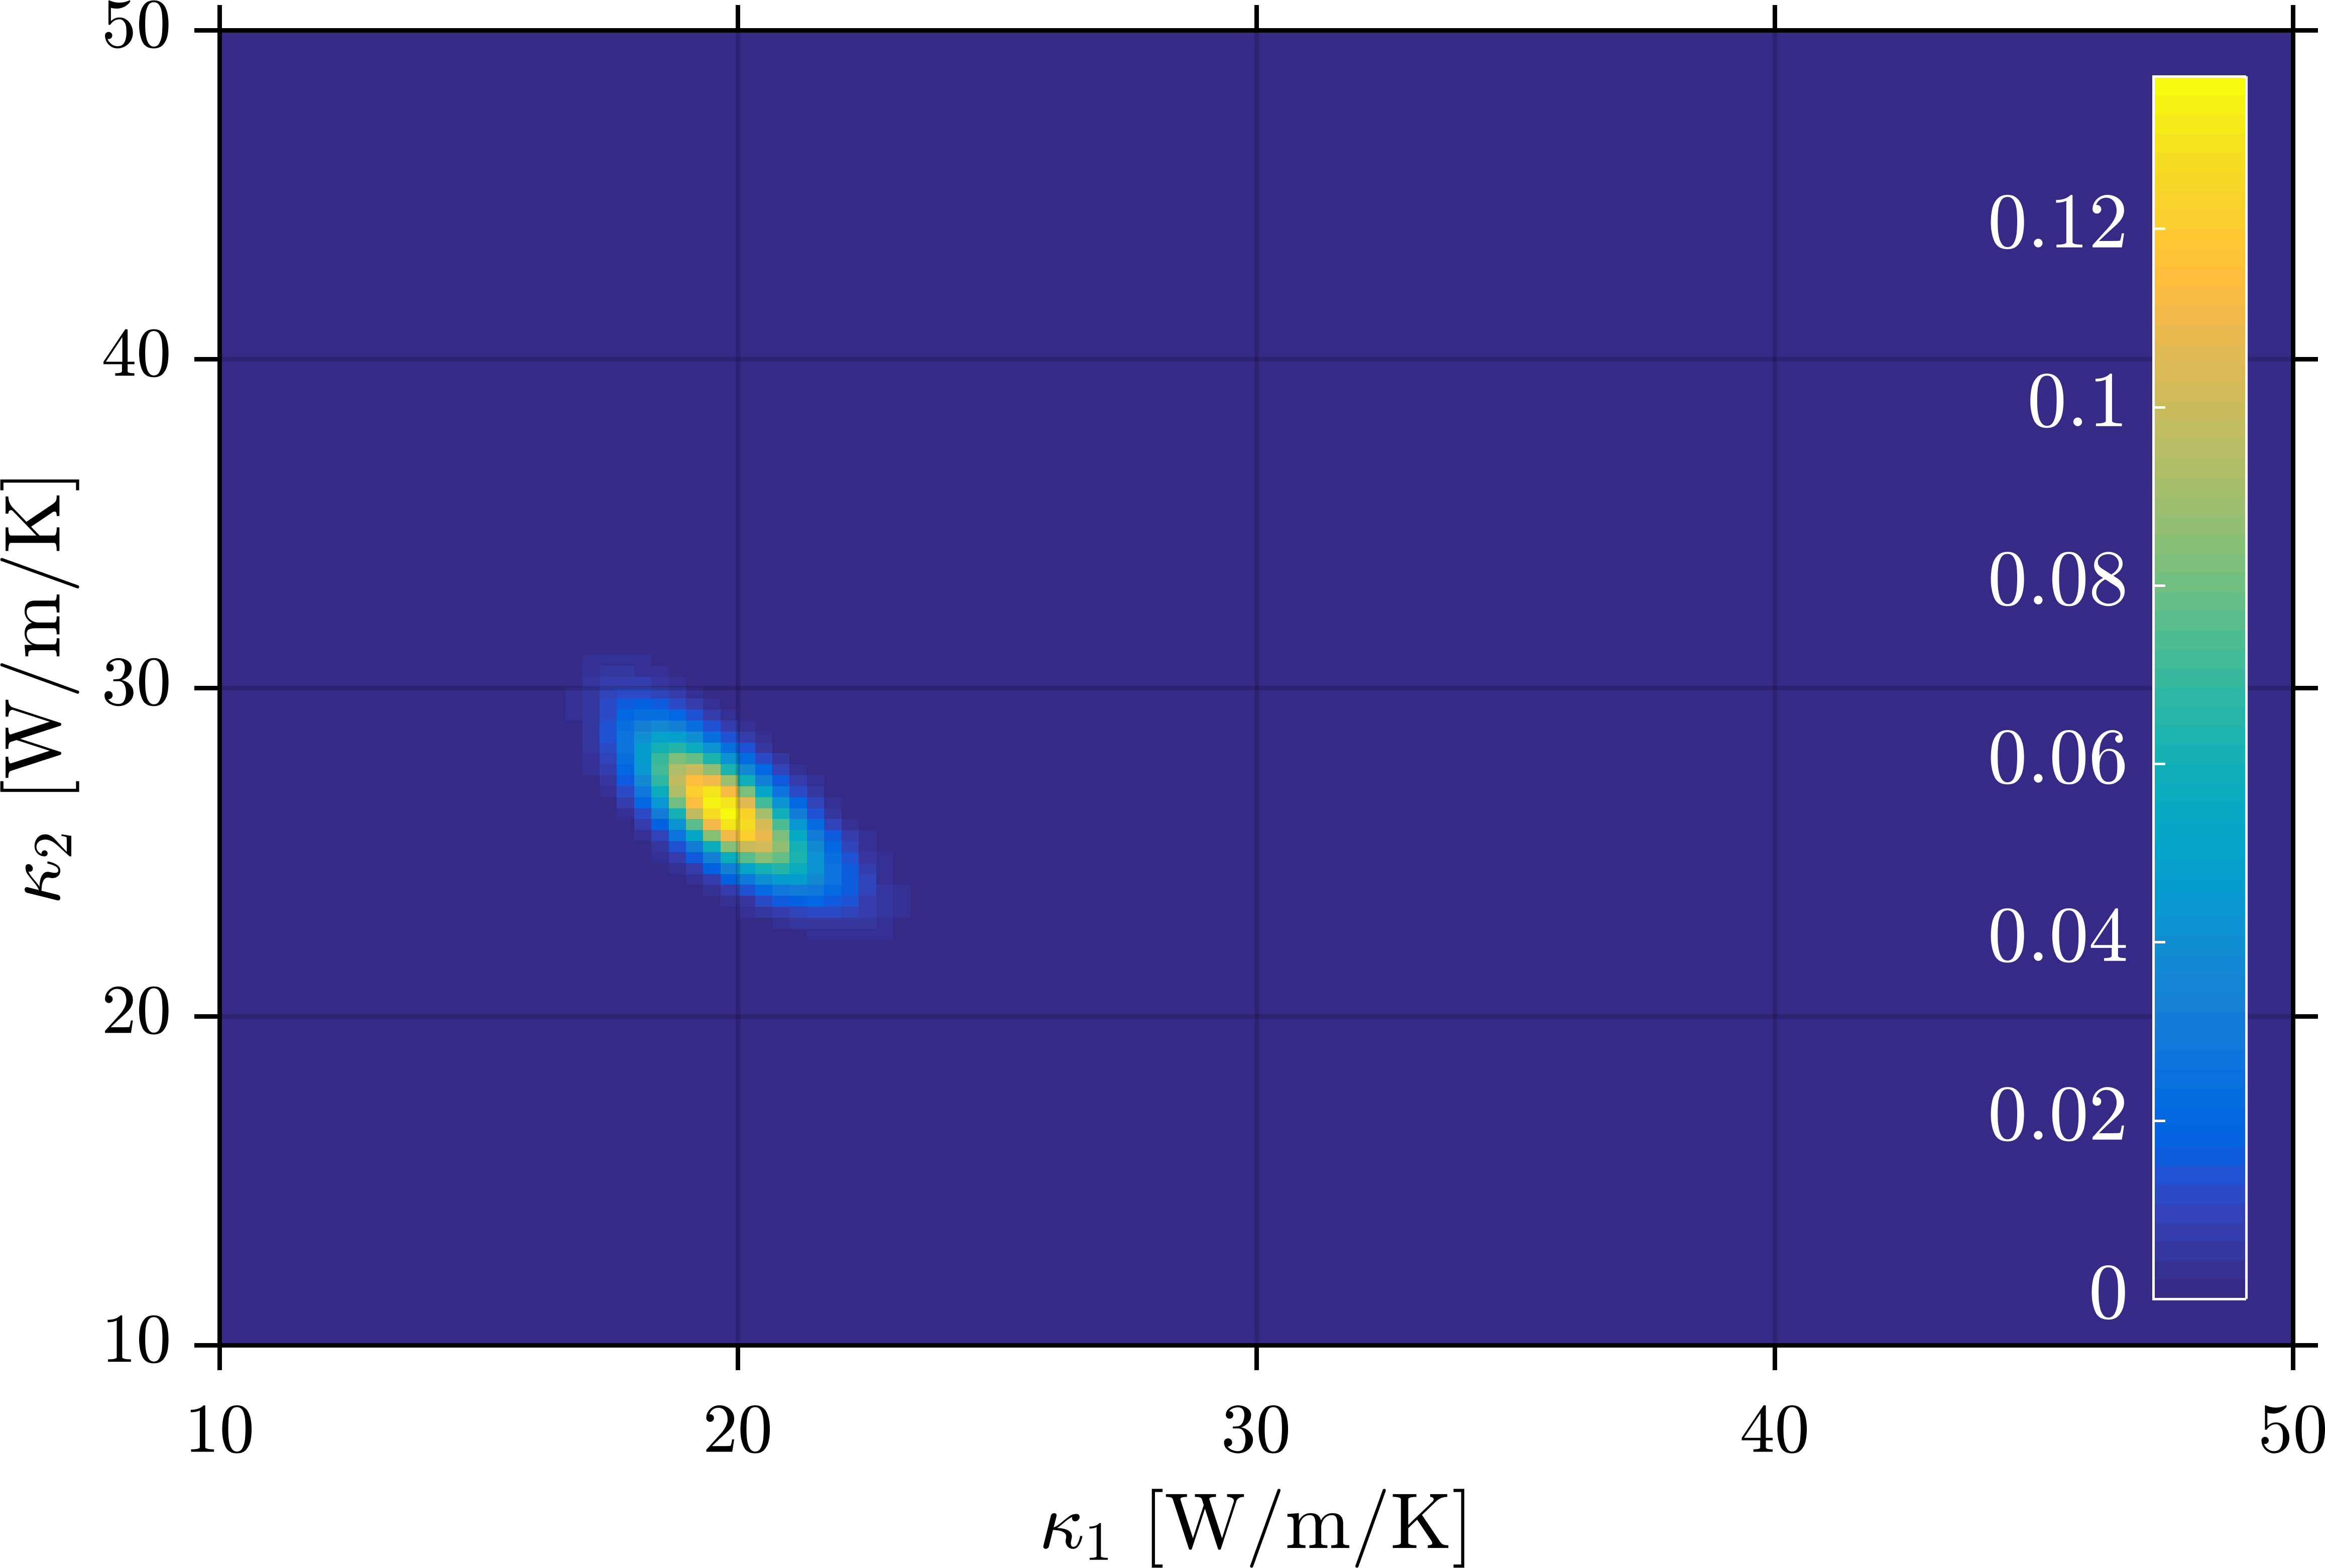
\includegraphics[height=\MAPfigHeight]{fig_Transport_Post2D_12_MCMC}
    \caption{MCMC.}
    \label{fig:Transport:Post:Marginals2D:12:MCMC}
  \end{subfigure}\hfill%
  \begin{subfigure}[b]{\MAPsubWidth}
    \centering
    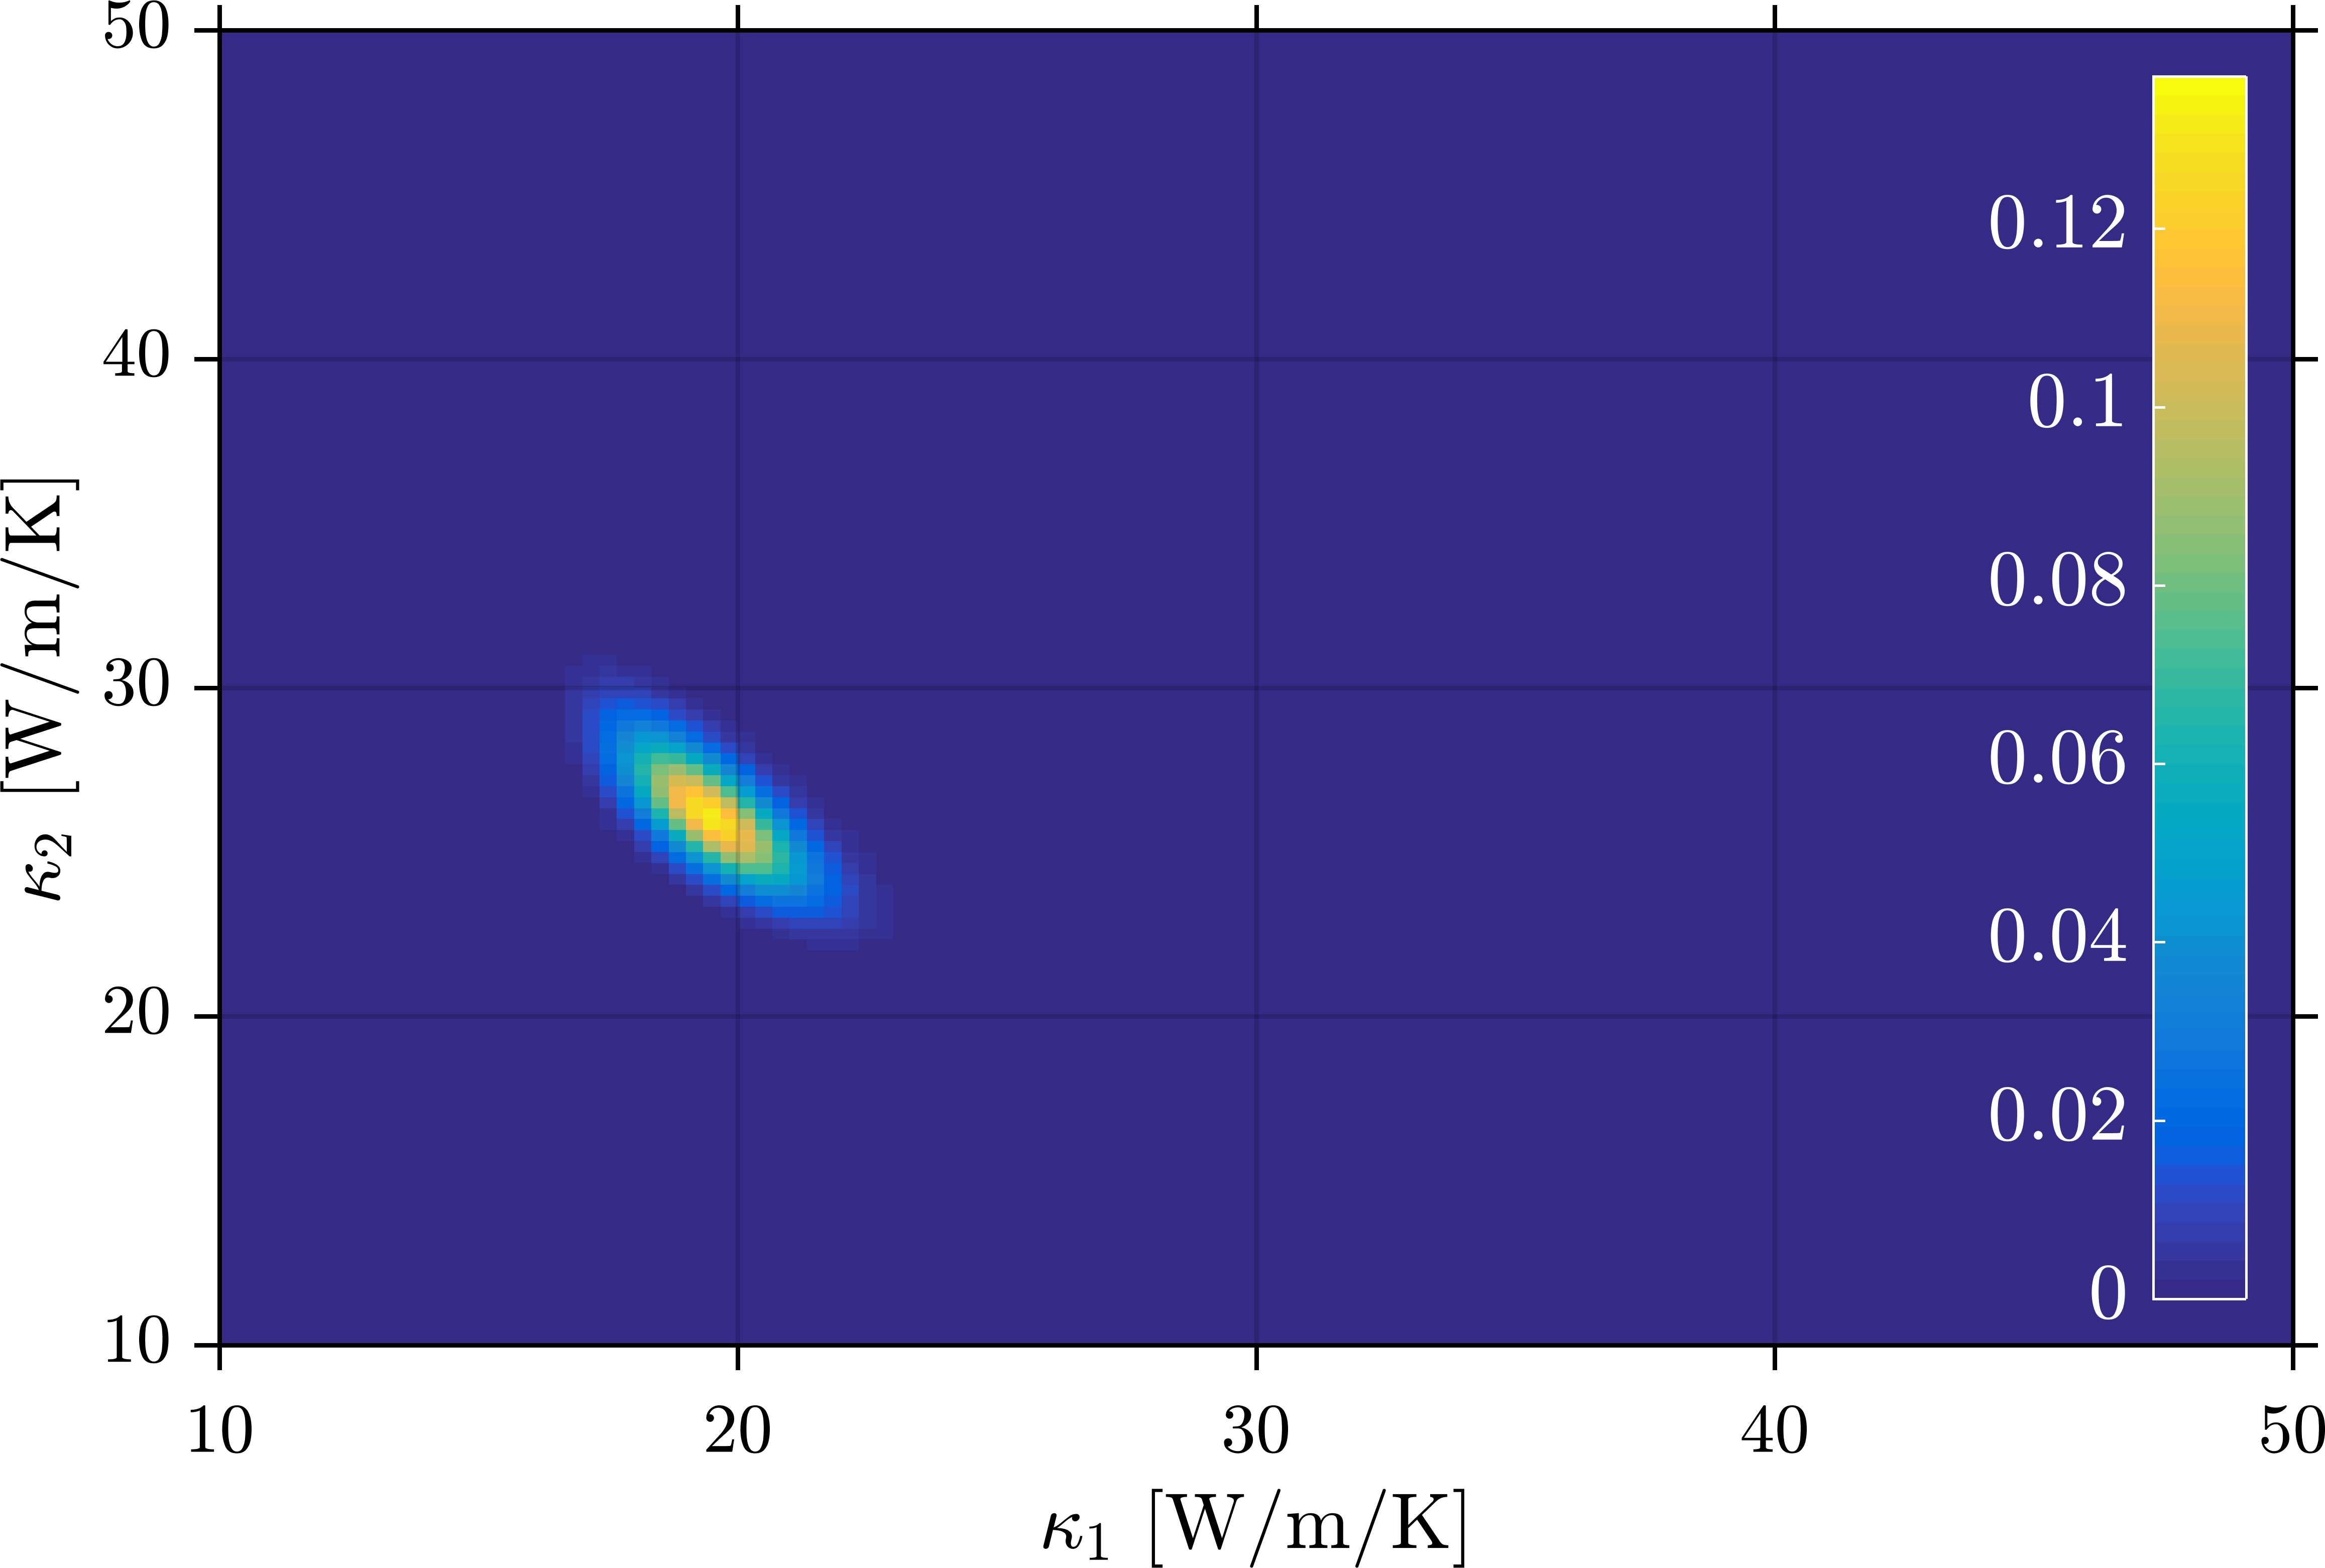
\includegraphics[height=\MAPfigHeight]{fig_Transport_Post2D_12_Map}
    \caption{Mapping.}
    \label{fig:Transport:Post:Marginals2D:12:Map}
  \end{subfigure}\\[3ex]%
  \begin{subfigure}[b]{\MAPsubWidth}
    \centering
    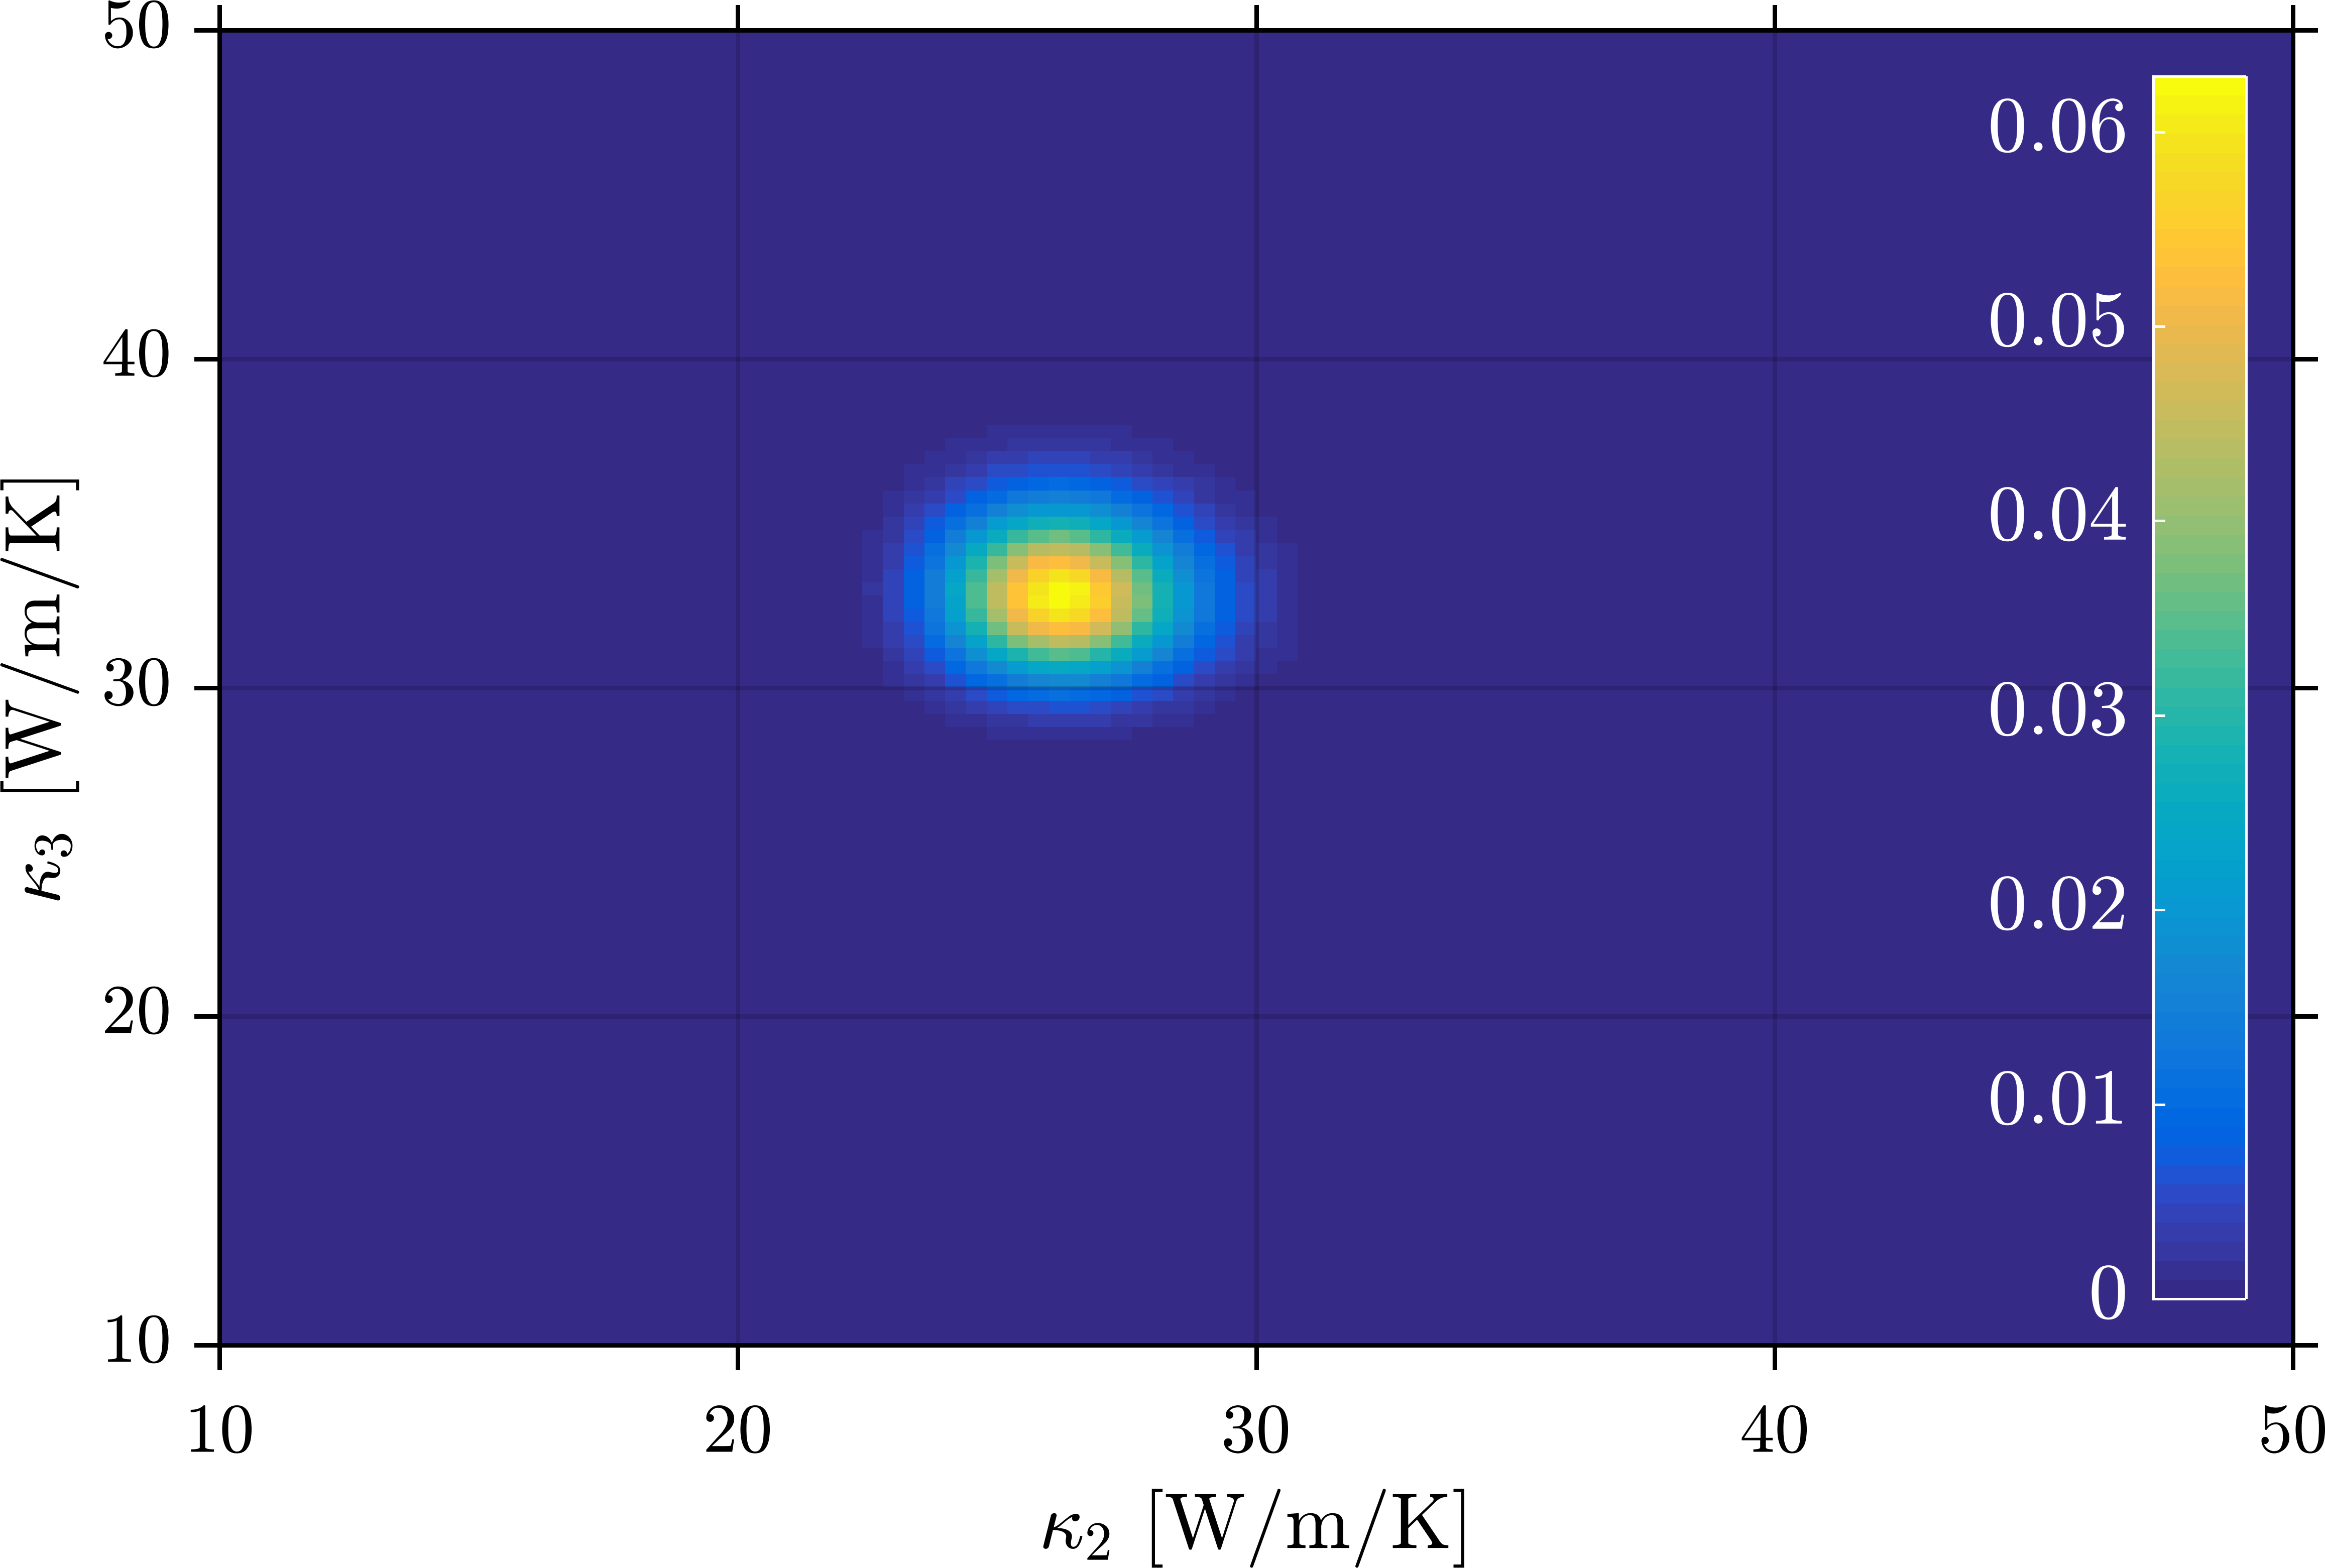
\includegraphics[height=\MAPfigHeight]{fig_Transport_Post2D_23_MCMC}
    \caption{MCMC.}
    \label{fig:Transport:Post:Marginals2D:23:MCMC}
  \end{subfigure}\hfill%
  \begin{subfigure}[b]{\MAPsubWidth}
    \centering
    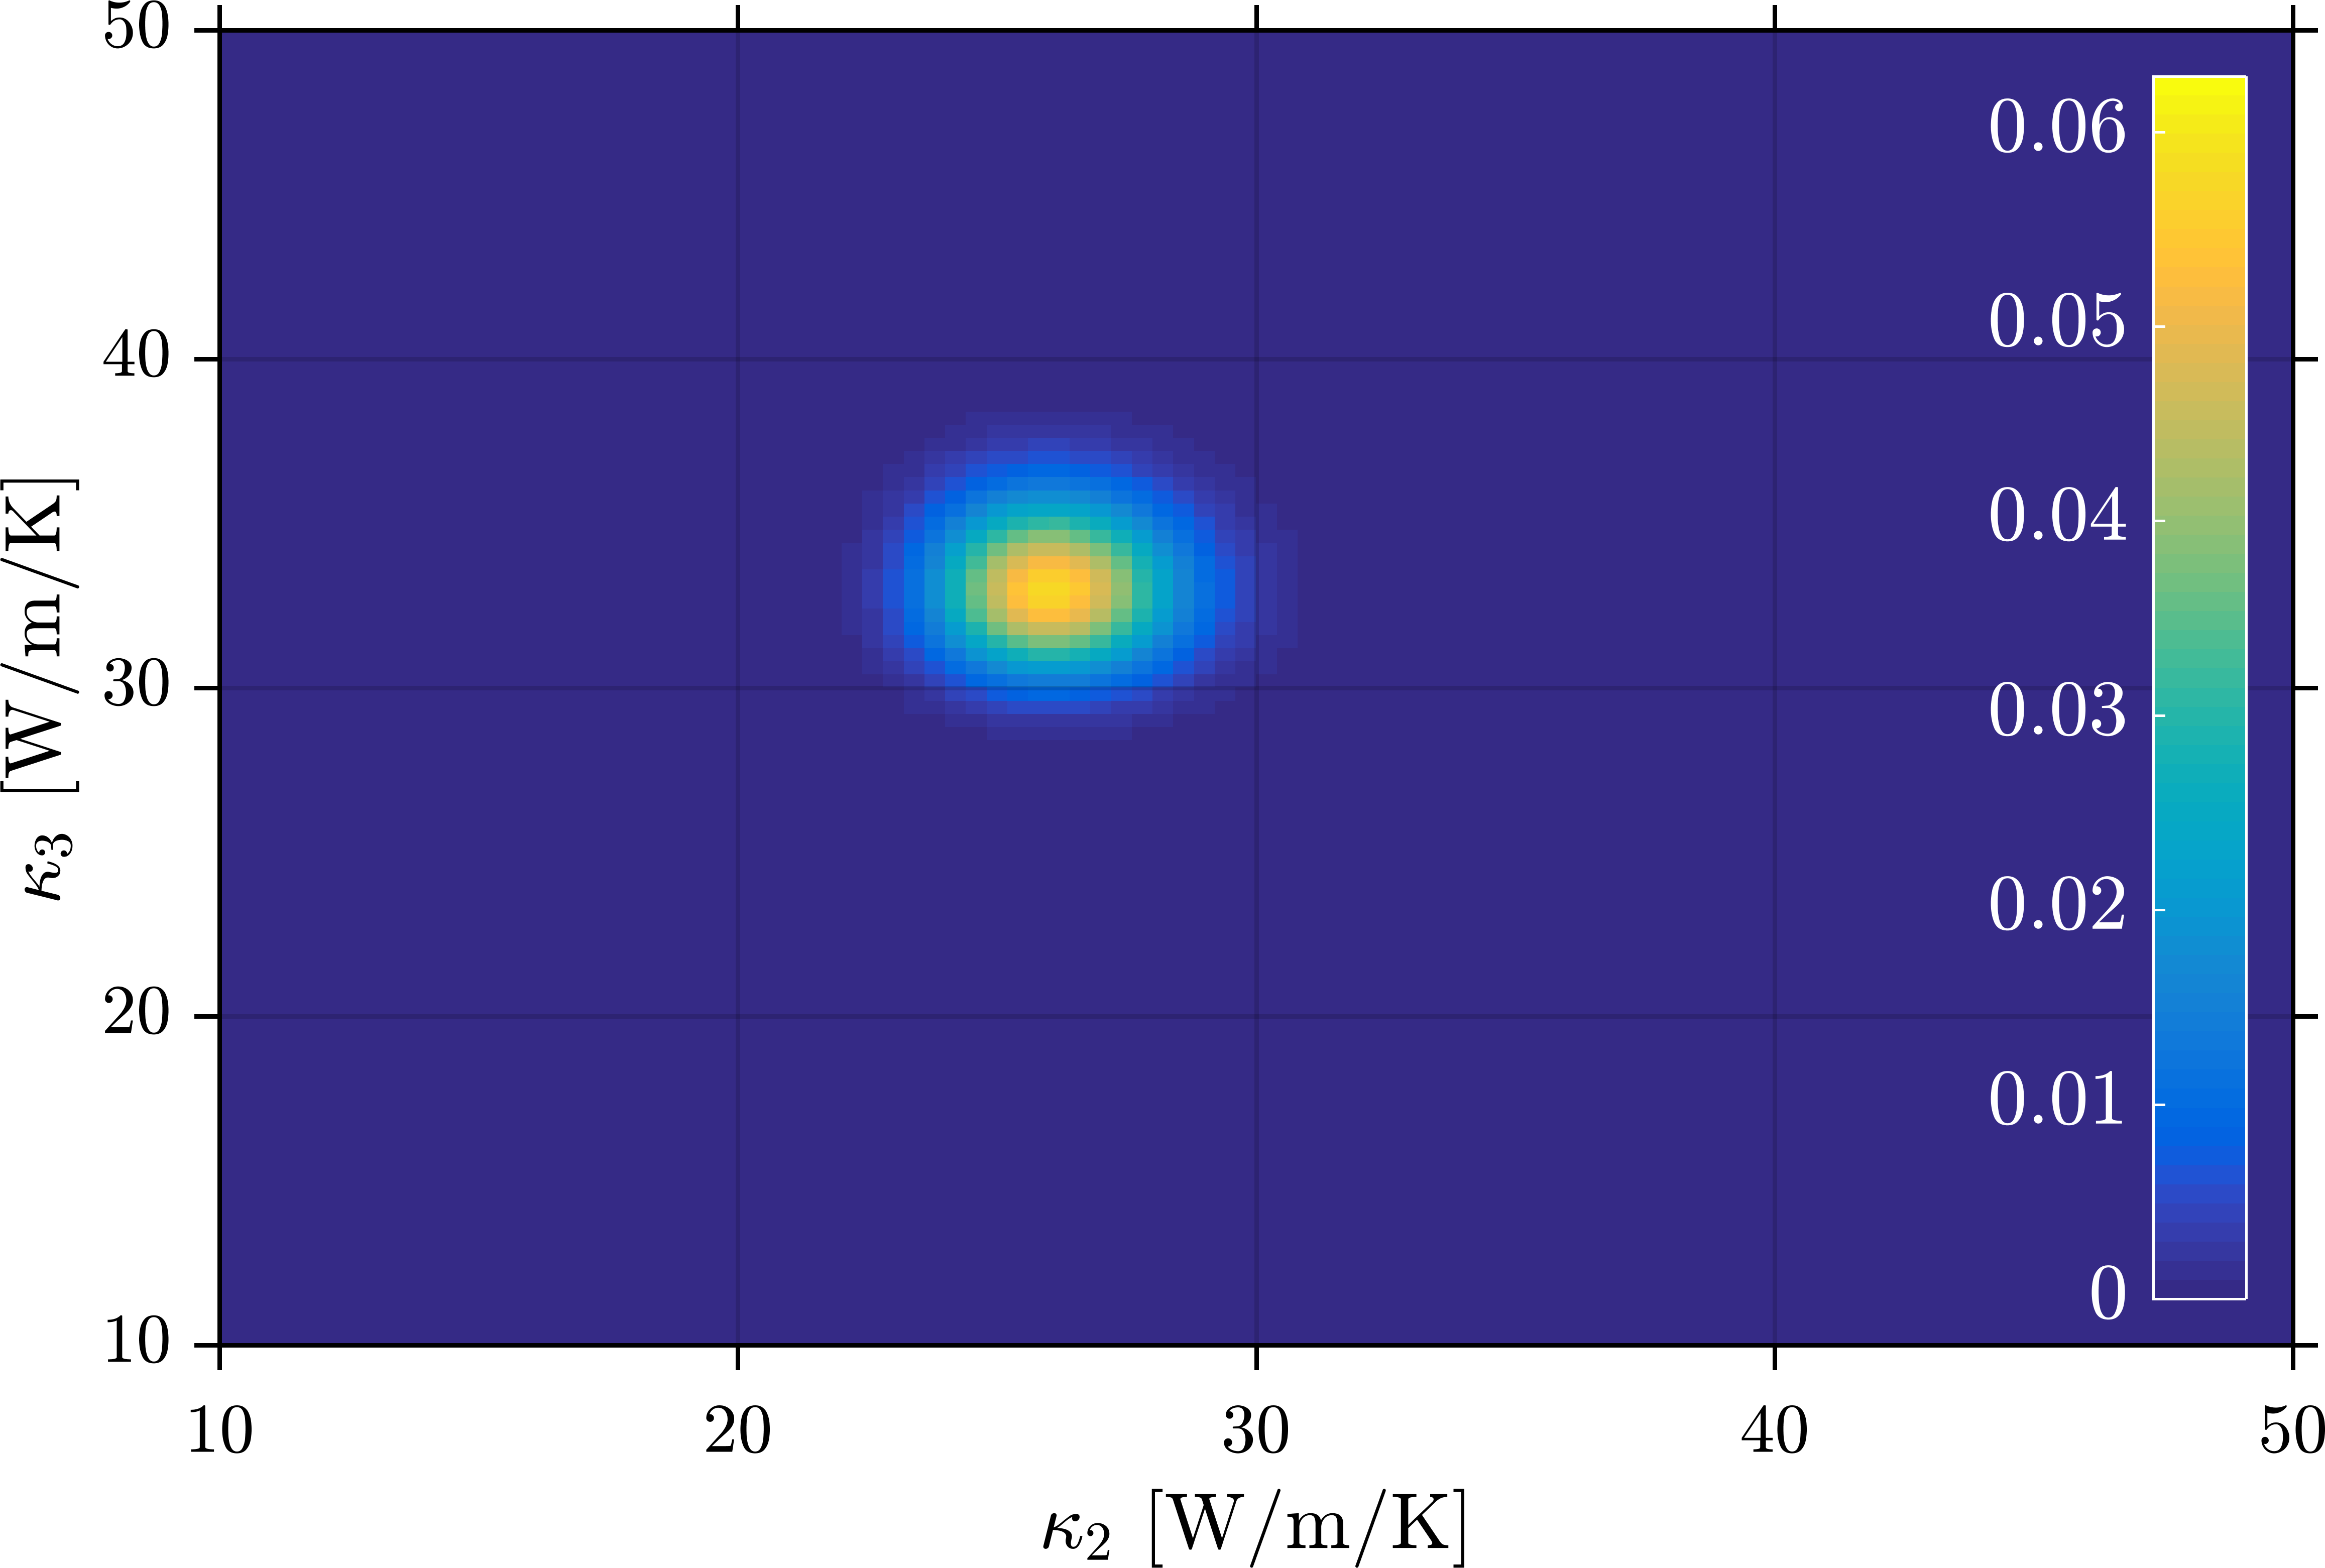
\includegraphics[height=\MAPfigHeight]{fig_Transport_Post2D_23_Map}
    \caption{Mapping.}
    \label{fig:Transport:Post:Marginals2D:23:Map}
  \end{subfigure}\\[3ex]%
  \begin{subfigure}[b]{\MAPsubWidth}
    \centering
    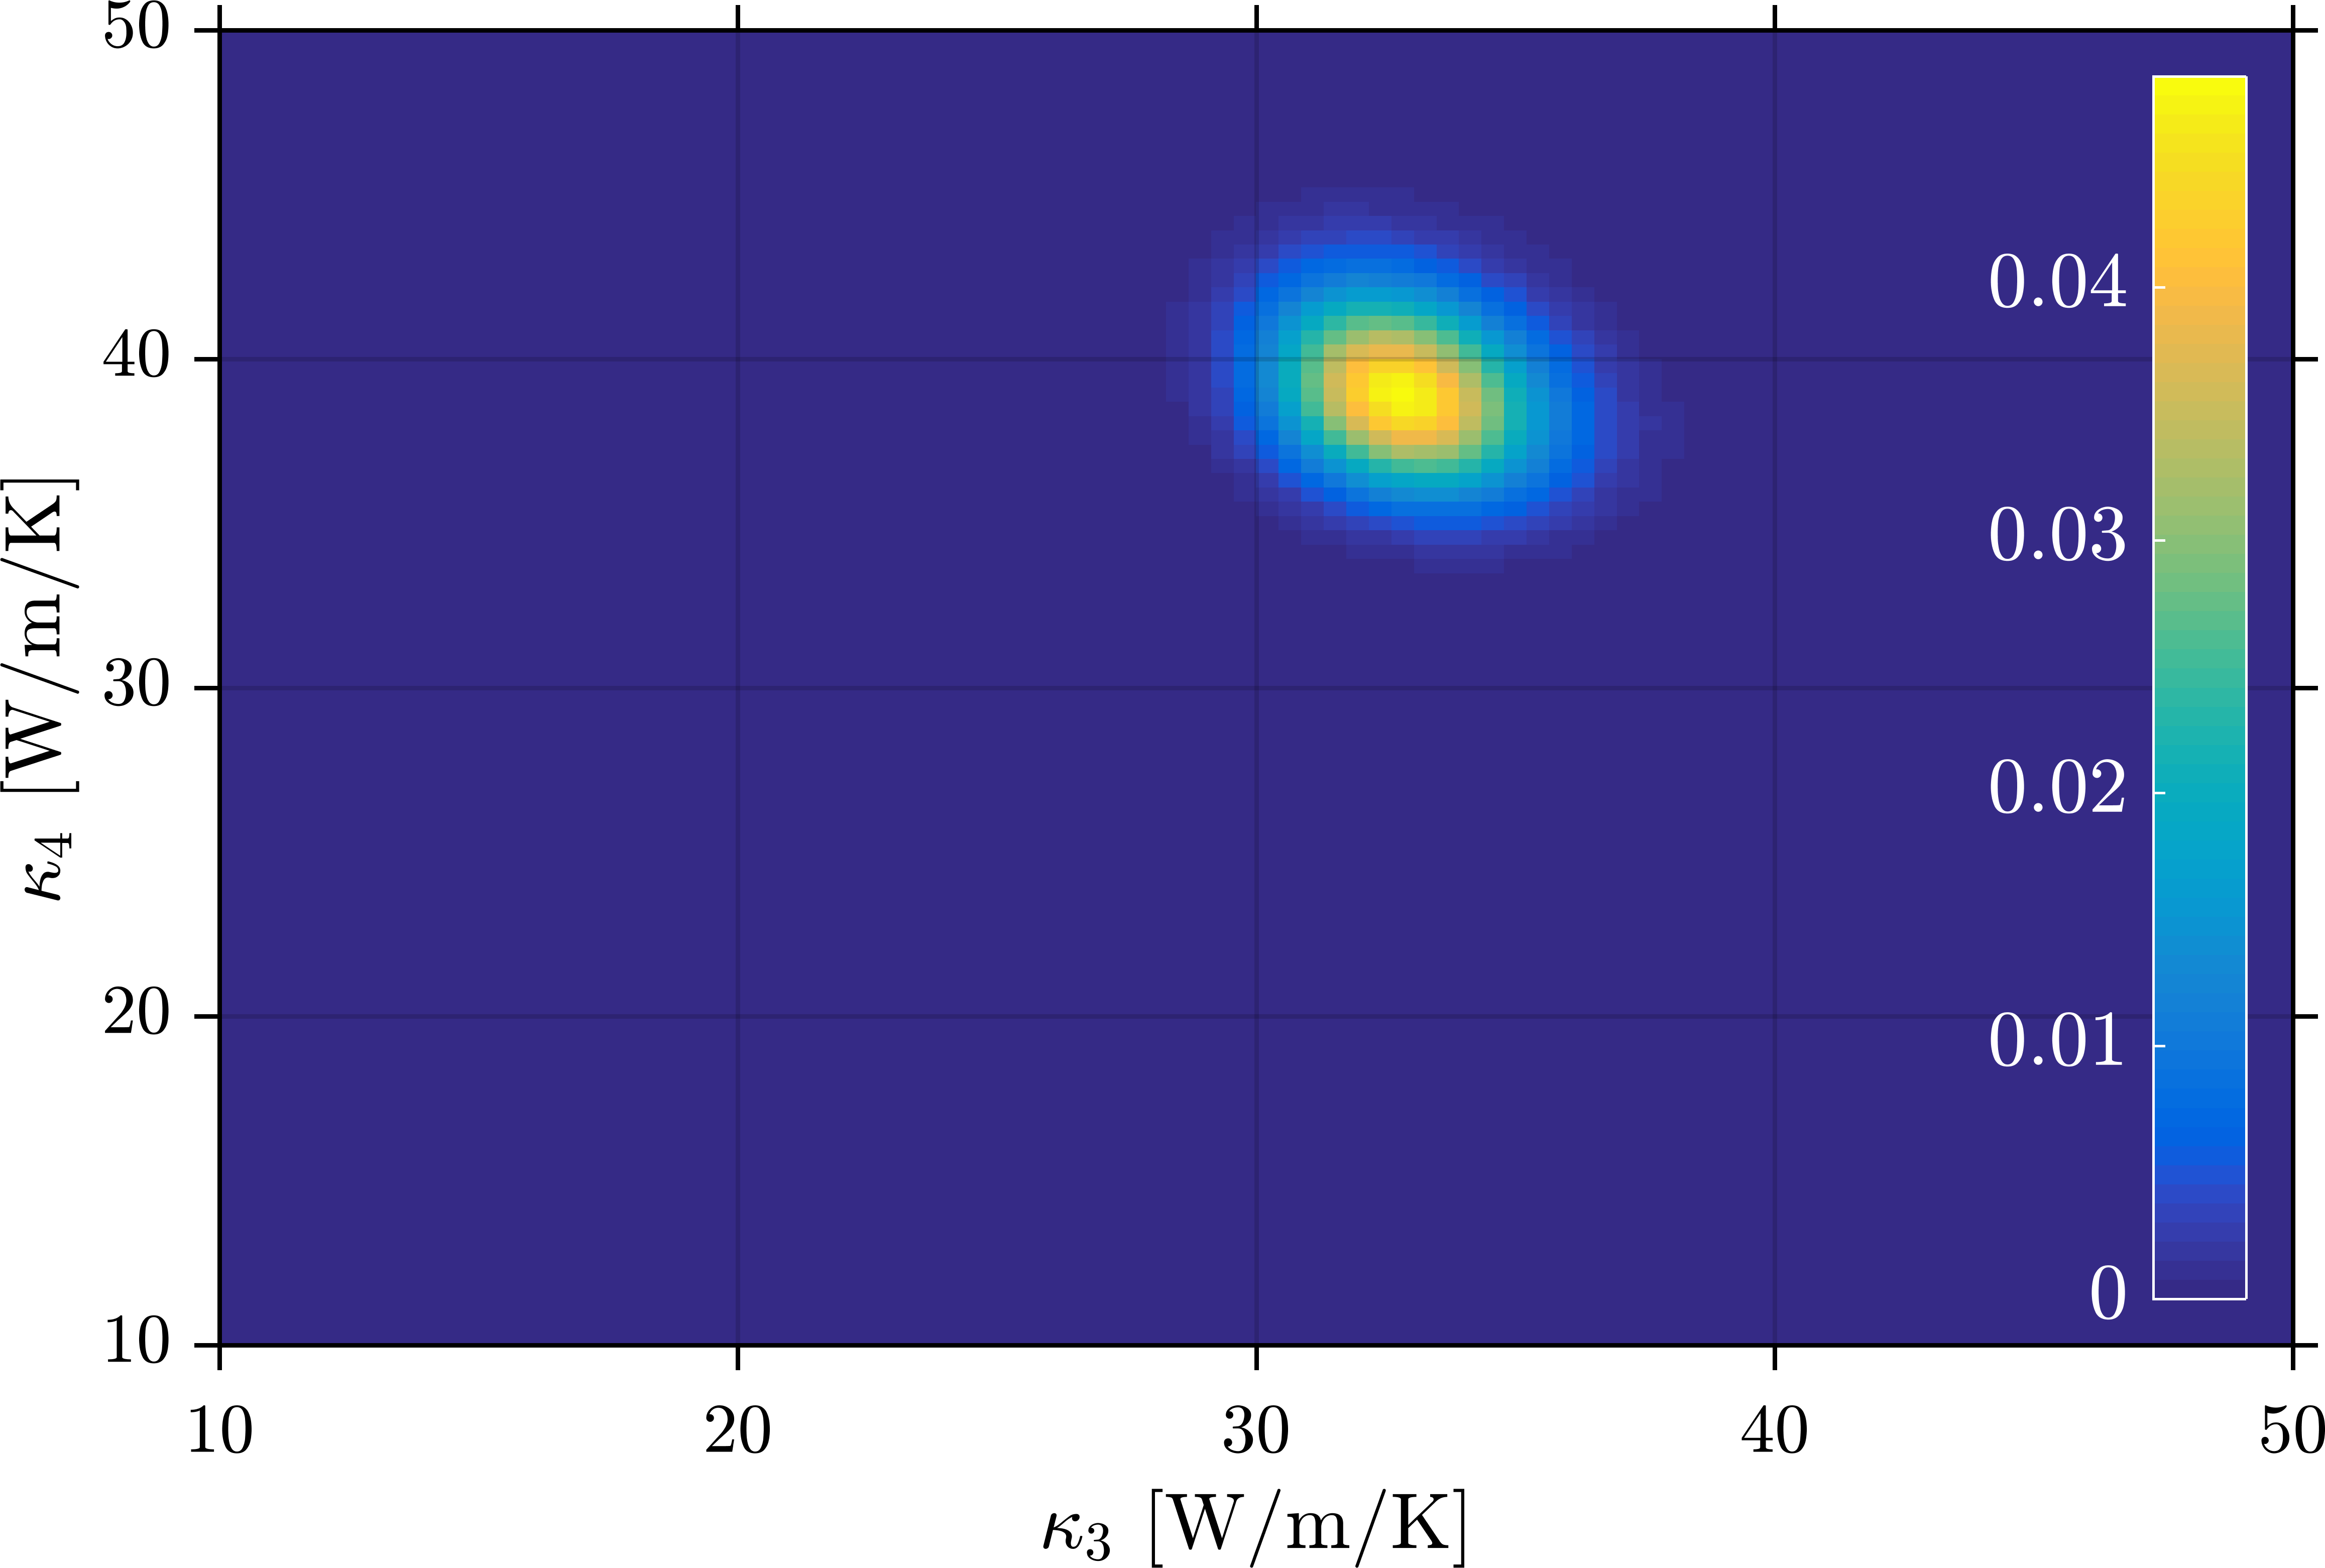
\includegraphics[height=\MAPfigHeight]{fig_Transport_Post2D_34_MCMC}
    \caption{MCMC.}
    \label{fig:Transport:Post:Marginals2D:34:MCMC}
  \end{subfigure}\hfill%
  \begin{subfigure}[b]{\MAPsubWidth}
    \centering
    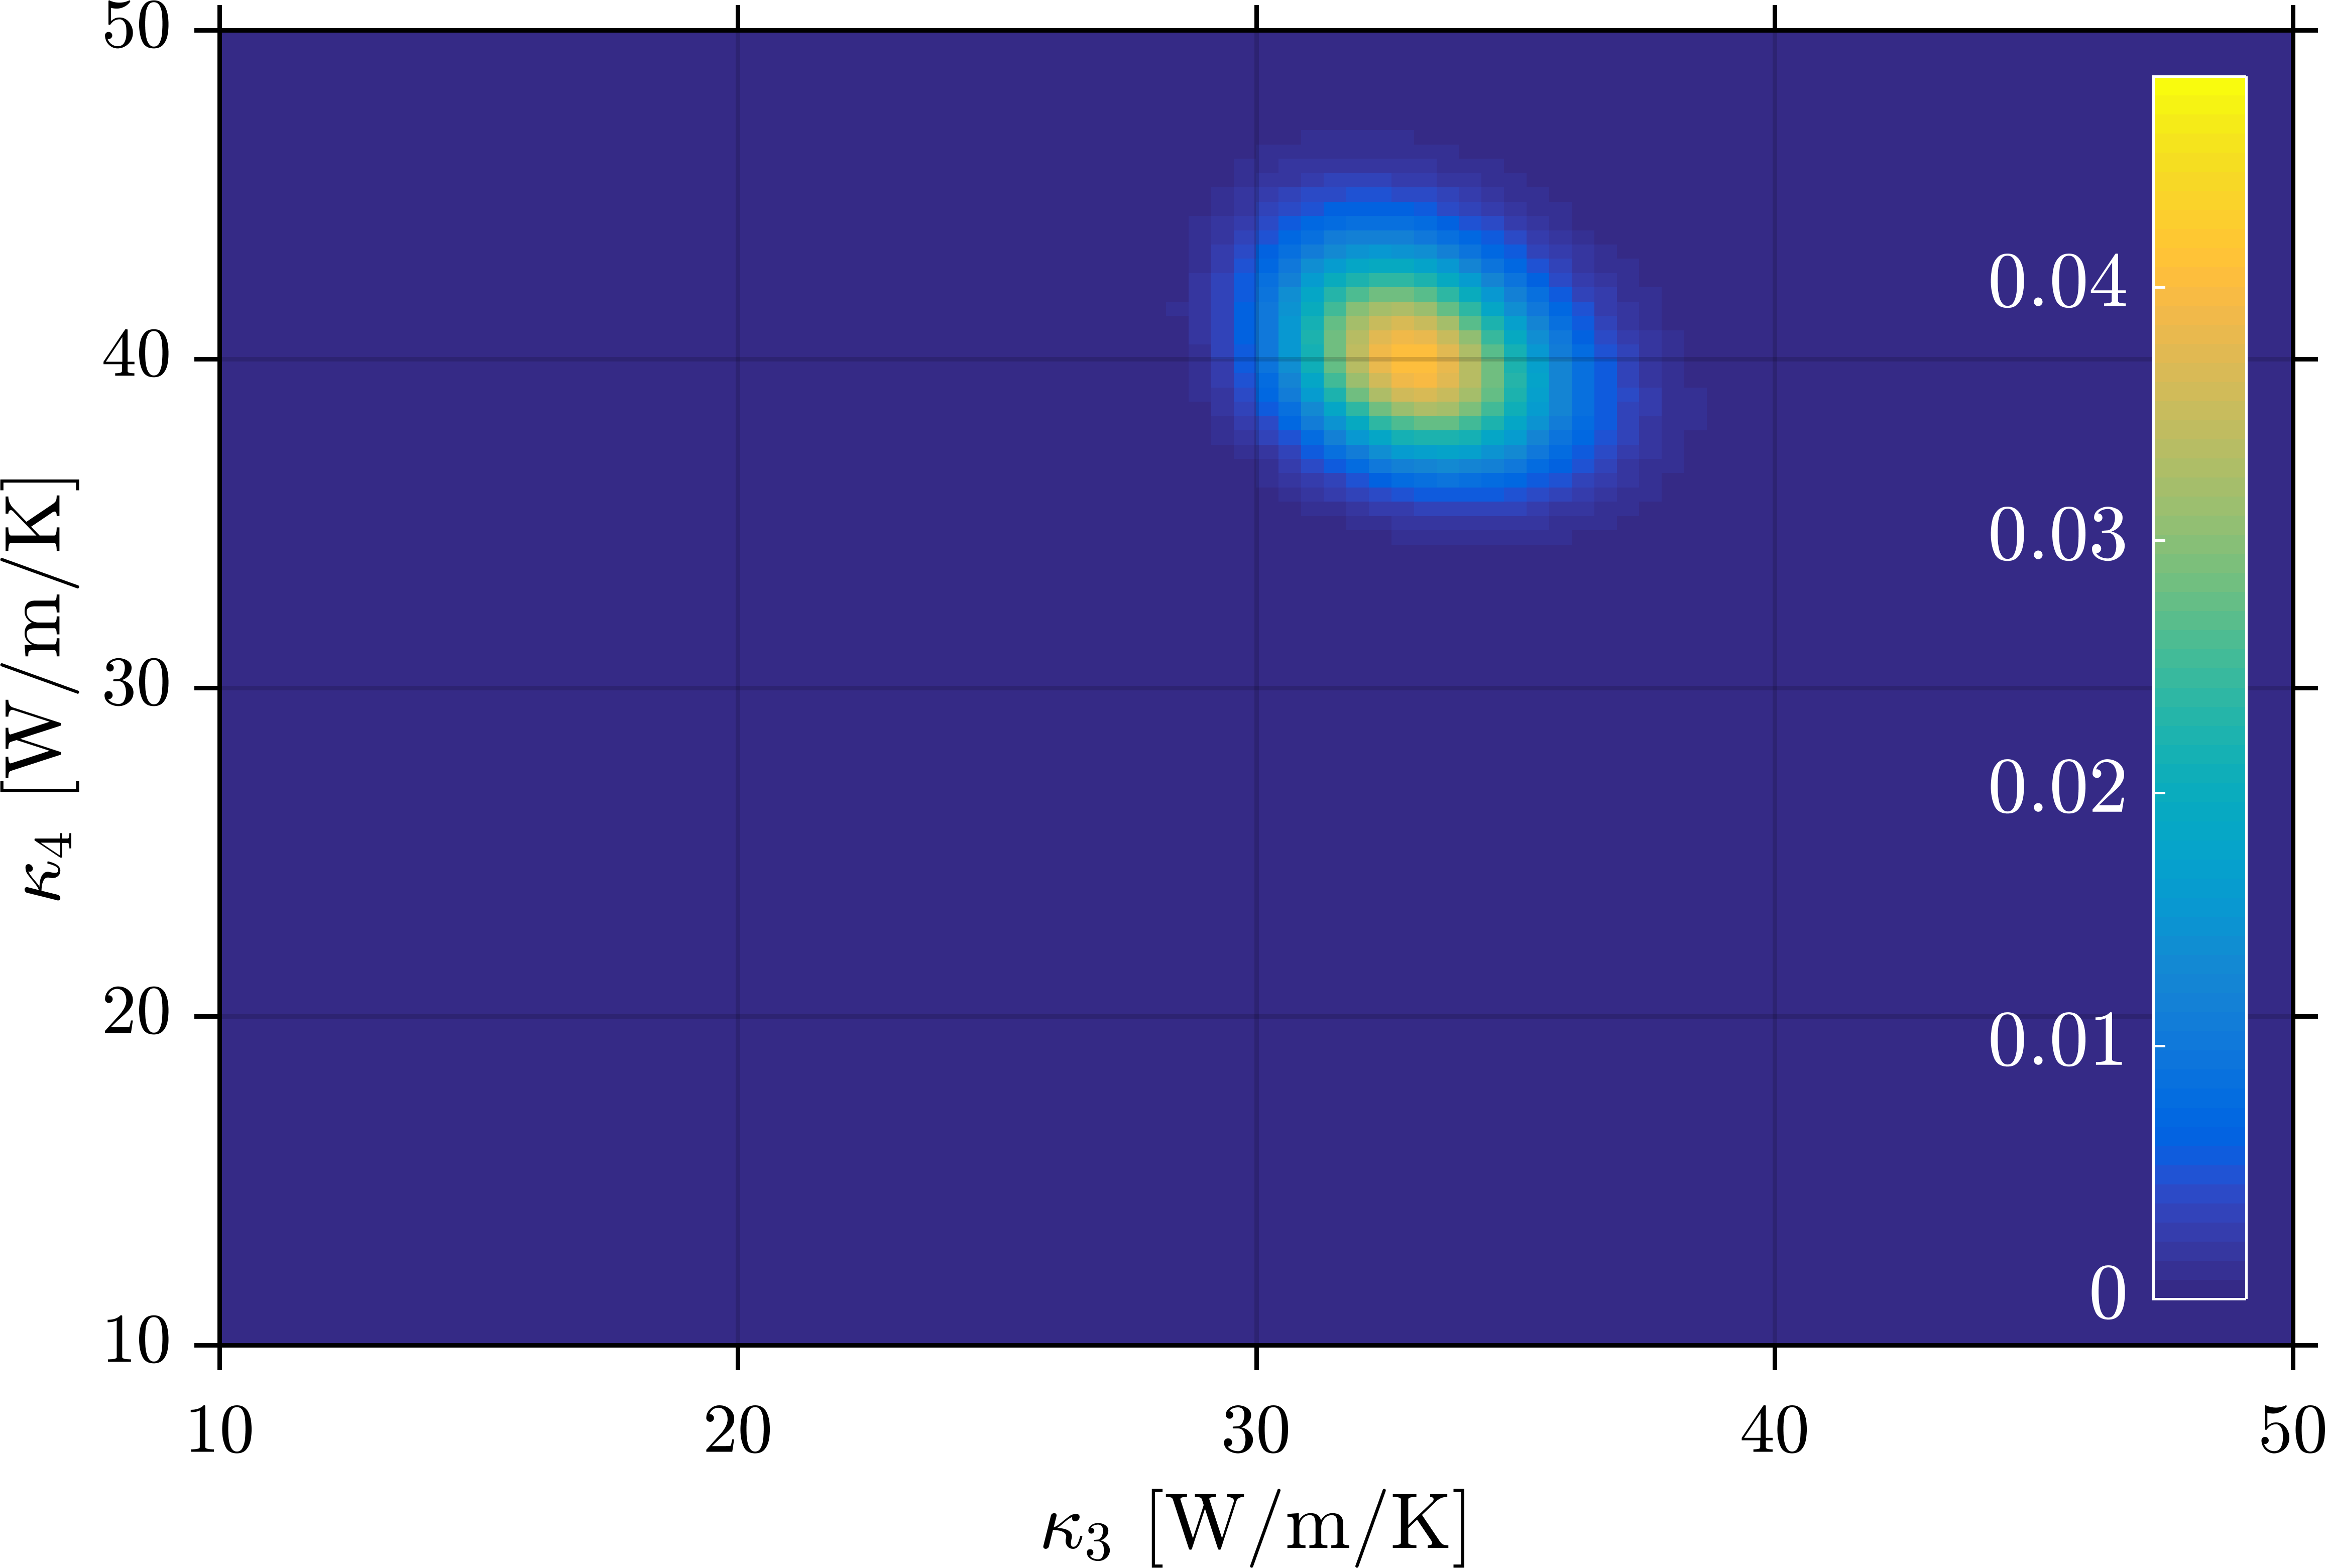
\includegraphics[height=\MAPfigHeight]{fig_Transport_Post2D_34_Map}
    \caption{Mapping.}
    \label{fig:Transport:Post:Marginals2D:34:Map}
  \end{subfigure}%
  \caption[Two-dimensional posterior marginals]{Two-dimensional posterior marginals.}
  \label{fig:Transport:Post:Marginals2D}
\end{figure}
\par % SIGN CONSIDERATIONS
The consideration of the sign of the Jacobian determinant in the course of the BFGS iterations \(\iota = 0,\ldots,I\) over the prior range provides some interesting insights.
We find that the Jacobian \(\det J_{\map^\vartriangle_{\hat{\bm{\coeffM}}}}(\bm{x}^{(l)}) < 0\) of the finally computed map is negative for all prior samples \(\bm{x}^{(l)}\) with \(l=1,\ldots,L\).
This indicates that the computed map \(\map^\vartriangle_{\hat{\bm{\coeffM}}}\) is indeed invertible over large proportions of the input space that are covered well by the prior.
One might think that this justifies \cref{eq:Transport:PriorTransformation,eq:Transport:PosteriorBacktransformation}, which only hold for invertible maps, in retrospect.
However, while the algorithm is initialized such that the Jacobian \(\det J_{\map^\vartriangle_{\bm{\coeffM}_0}} > 0\) is positive in the beginning,
it takes on positive and negative values \(\det J_{\map^\vartriangle_{\bm{\coeffM}_\iota}} \gtrless 0\) after some intermediary iterations.
For such intermediate maps, the Jacobian determinant has zeros in regions of the parameter space that accumulate most prior mass.
This signifies that these maps cannot be inverted globally.
\par % STATISTICAL SUMMARIES
The transformation and the MCMC results can be also compared by reference to the first posterior moments.
In \cref{tab:Transport:Post:Summaries} the conditional means, standard deviations and linear correlations are summarized in tabular form.
Apart from the correlation coefficients, all results are given in units of \([\kappa] = \unit[]{W/m/K}\).
While the MCMC reference values are statistical sample approximations, transformation-based inference allows us to calculate
the moments from the coefficients of the transport map through \cref{eq:Transport:OutputMeanVariance,eq:Transport:OutputCovariance}.
It is seen that the transportation manages to characterize the posterior in terms of its first statistical moments.
The expected values \(\mathds{E}[\kappa_i \cond \bm{y}]\) are reproduced satisfactorily for \(i=1,\ldots,4\).
As measured by the standard deviations \(\mathrm{Std}[\kappa_i \cond \bm{y}] = \mathrm{Var}[\kappa_i \cond \bm{y}]^{1/2}\),
the transformed distribution tends to overestimate the spread of the posterior slightly.
The correlations \(\rho[\kappa_i,\kappa_j \cond \bm{y}] = \mathrm{Cov}[\kappa_i,\kappa_j \cond \bm{y}] / \mathrm{Std}[\kappa_i \cond \bm{y}] / \mathrm{Std}[\kappa_j \cond \bm{y}]\)
for \(i,j=1,\ldots,4\) are captured well.
We conclude that, all in all, the prior has been successfully transformed into the posterior by the low-order transport map.
% TABLE: STATISTICAL QUANTITIES
\begin{table}[htbp]
  \caption[Posterior summaries]{Posterior summaries.}
  \label{tab:Transport:Post:Summaries}
  \centering
  \begin{tabular}{lccccccc}
    \toprule
    & \(\mathds{E}[\kappa_1 \cond \bm{y}]\) & \(\mathds{E}[\kappa_2 \cond \bm{y}]\) & \(\mathds{E}[\kappa_3 \cond \bm{y}]\) & \(\mathds{E}[\kappa_4 \cond \bm{y}]\)
    & \(\mathrm{Std}[\kappa_1 \cond \bm{y}]\) & \(\mathrm{Std}[\kappa_2 \cond \bm{y}]\) & \(\mathrm{Std}[\kappa_3 \cond \bm{y}]\) \\
    \midrule
    MCMC    & \(19.78\) & \(26.36\) & \(32.94\) & \(39.06\) & \(1.11\) & \(1.50\) & \(1.69\) \\
    Mapping & \(19.52\) & \(26.18\) & \(33.16\) & \(40.18\) & \(1.12\) & \(1.55\) & \(1.78\) \\
    \midrule
    & \(\mathrm{Std}[\kappa_4 \cond \bm{y}]\) & \(\rho[\kappa_1,\kappa_2 \cond \bm{y}]\) & \(\rho[\kappa_1,\kappa_3 \cond \bm{y}]\) & \(\rho[\kappa_1,\kappa_4 \cond \bm{y}]\)
    & \(\rho[\kappa_2,\kappa_3 \cond \bm{y}]\) & \(\rho[\kappa_2,\kappa_4 \cond \bm{y}]\) & \(\rho[\kappa_3,\kappa_4 \cond \bm{y}]\) \\
    \midrule
    MCMC    & \(2.01\) & \(-0.38\) & \(-0.22\) & \(-0.02\) & \(-0.03\) & \(-0.72\) & \(-0.36\) \\
    Mapping & \(2.25\) & \(-0.39\) & \(-0.24\) & \(-0.01\) & \(-0.01\) & \(-0.72\) & \(-0.38\) \\
    \bottomrule
  \end{tabular}
\end{table}
\par % MODEL EVIDENCE
Lastly we investigate the model evidence \(\scale\).
It can be estimated by brute-force MC simulation on the one hand.
On the other hand, one may use the relation \(\scale \geq \exp(\mathcal{G}(\map))\) that emerged in the context of
\cref{eq:Transport:FreeEnergy,eq:Transport:MinimizeKullbackLeibler} in order to approximate the model evidence.
After maximizing the sample average function in \cref{eq:Transport:SampleAverageFunction} as described by \cref{eq:Transport:OptimizationSAA},
\(\scale \approx \exp(\hat{\mathcal{G}}(\hat{\bm{\coeffM}}))\) may serve as a biased estimator of the model evidence.
The convergence of this quantity in the optimization was already monitored in \cref{tab:Transport:BFGS:Convergence}.
With the abovementioned procedures, the model evidence is determined as \(\scale_{\mathrm{MC}} = 1.97 \times 10^{-5}\)
and \(\scale_{\mathrm{Map}} = \exp(\hat{\mathcal{G}}(\hat{\bm{\coeffM}})) = 9.86 \times 10^{-5}\).
Even though \(\exp(\mathcal{G}(\map))\) establishes a lower bound of the evidence in theory,
\(\exp(\hat{\mathcal{G}}(\hat{\bm{\coeffM}}))\) practically overestimates the MC reference solution.
Contrary to the estimation of the first posterior moments that works rather well, the computation of the model evidence in inferential transportation seems to be more problematic.